% REMEMBER: You must not plagiarise anything in your report. Be extremely careful.

\documentclass{l4proj}

    
%
% put any additional packages here
%
\renewcommand\floatpagefraction{.9}
\renewcommand\topfraction{.9}
\renewcommand\bottomfraction{.9}
\renewcommand\textfraction{.1}   
\setcounter{totalnumber}{50}
\setcounter{topnumber}{50}
\setcounter{bottomnumber}{50}
\usepackage{pdfpages}

\begin{document}

%==============================================================================
%% METADATA
\title{Gone Phishing: A Context Relevant Anti-Phishing Training Game }
\author{Joel Feven}
\date{April 21, 2022}

\maketitle

%==============================================================================
%% ABSTRACT
\begin{abstract}

Phishing and data theft are major issues in cyber-security in the modern age. As algorithms and security software improves, hackers often resort to targeting the user of the system rather than the system itself, this is known as phishing. Protecting users against phishing attacks can be a very difficult task, especially in the case of spear-phishing, in which specific individuals are targeted and sent context relevant phishing emails that are almost undetectable. As a result, user must be prepared to deal with such attacks through training. This project will attempt to train users in both low level (no context) and high level (context heavy) phishing attacks through a simulated email client. The users will have to navigate and detect phishing emails as they are received in each of the levels. The users are then scored on their effectiveness and efficiency. After fully evaluating and testing the application, it was found that the training did improve the average detection rate and phishing knowledge of users.

\end{abstract}

%==============================================================================

% EDUCATION REUSE CONSENT FORM
% If you consent to your project being shown to future students for educational purposes
% then insert your name and the date below to  sign the education use form that appears in the front of the document. 
% You must explicitly give consent if you wish to do so.
% If you sign, your project may be included in the Hall of Fame if it scores particularly highly.
%
% Please note that you are under no obligation to sign 
% this declaration, but doing so would help future students.
%
%\def\consentname {My Name} % your full name
%\def\consentdate {20 March 2018} % the date you agree
%
\educationalconsent


%==============================================================================
\tableofcontents

%==============================================================================
%% Notes on formatting
%==============================================================================
% The first page, abstract and table of contents are numbered using Roman numerals and are not
% included in the page count. 
%
% From now on pages are numbered
% using Arabic numerals. Therefore, immediately after the first call to \chapter we need the call
% \pagenumbering{arabic} and this should be called once only in the document. 
%
% The first Chapter should then be on page 1. You are allowed 40 pages for a 40 credit project and 20 pages for a 
% 20 credit report. This includes everything numbered in Arabic numerals (excluding front matter) up
% to but excluding the appendices and bibliography.
%
% You must not alter text size (it is currently 10pt) or alter margins or spacing.
%
%
%==================================================================================================================================
%
% IMPORTANT
% The chapter headings here are **suggestions**. You don't have to follow this model if
% it doesn't fit your project. Every project should have an introduction and conclusion,
% however. 
%
%==================================================================================================================================
\chapter{Introduction}

\section{Motivation}

With the rise of technology in all aspects of society, security has become a major concern for many. Due to the amount of data stored on databases and online, personal data is easier than ever to steal. Phishing is one of the many practices used by cyber-criminals to infiltrate and steal data from both average people and large institutions and businesses alike. The main challenge that people face is the lack of awareness or knowledge on how to deal with phishing attacks. Therefore, anti-phishing training is critical in the safety of all members of society and business. However, the ever-fluctuating deception and manipulation techniques used by cyber-criminals make effective training difficult to employ on a large scale. These techniques often use social engineering to intercept and impersonate others (context) in the attacks, making context-based phishing very difficult to detect.

\section{Aims}
This project aims to create an application to:
\begin{itemize}
    \item Train users to effectively detect and avoid phishing attacks
    \item Inform users of techniques used by phishers
    \item easily use on a number of devices
    \item Employ context and immersion in the training process
\end{itemize}

\section{Structure}
This dissertation is structured in the following manner:
\begin{itemize}
    \item Chapter 2: Background of phishing and training materials, with exploration of existing systems.
    \item Chapter 3: Analysis and Requirements required for this system, developed from the prior chapters.
    \item Chapter 4: Design of the system in both back-end and front-end, including wireframes and features.
    \item Chapter 5: Implementation process of the system along with the technologies used.
    \item Chapter 6: Evaluation of the final system through both unit testing and user evaluation
    \item Chapter 7: Conclusion summarising the project as a whole with reflections and reference to future work.
\end{itemize}

% reset page numbering. Don't remove this!
\pagenumbering{arabic} 



%==================================================================================================================================
\chapter{Background}

This chapter explores phishing and methods used by phishers. It also explores the effectiveness of training materials and the requirements for such training. The final section of this chapter analyses the existing applications that have attempted anti-phishing training.

\section{What is Phishing?}
With the rise of technology and computer-based solutions, the vast majority of corporations around the world rely on computers for data storage, analysis, and communication. However, this has one fatal flaw: \textit{people} are required to operate the vast majority of this technology. This has led to a large number of cyber-attacks directed towards the person behind the screen rather than the device itself, mainly through an attack known as “phishing”. The huge scale of the problem is shown by Oest et al. who states that between 2016-2017 over 1.9 billion user credentials were stolen through means of phishing \citep{oest2018inside}.

Phishing is a type of attack that makes use of social engineering to coerce users into giving personal information over to these attackers, known as “phishers”. As Parsons et al. finds, phishers make use of social engineering to convince a victim that they are legitimate and trustworthy in order to extract information or carry out further attacks \citep{parsons2019predicting}. This can be done with varying degrees of complexity, from generic widespread “spam” emails to user specific, personalised attacks (also known as “spear phishing”). 

When spear phishing targets a highly influential person within a company (or an employee with access to a large amount of data/information), this can be known as “whaling” due to the potentially large return of data/credentials/access from the company. In Q4 2016, the Anti-Phishing Working Group (APWG) found that each month there were around 90,000 phishing attacks, an increase of 5753\% of average phishing attacks from the last 12 years \citep{apwg2017phishing}. However, phishing is not limited to emails. It can be performed in a wide variety of methods and on different platforms such as social media and instant messaging services. As long as the user is exploited to perform an action or relay sensitive information, the attack is considered a phishing attack.

\subsection{Why is Phishing Worth Investigating?}
Phishing is a large problem. The Security Boulevard phishing report stated that around 88\% of the organisations monitored reported spear-phishing attacks \citep{bhardwaj2020phishing}. This goes to show that phishing is widespread and (due to the rising technological infrastructure requirement) commonplace in many businesses and industries. Therefore it is key to train \textbf{all} employees and freelancers in techniques to combat phishing attacks, no matter their technological skillset. Those without prior knowledge of phishing are often the easiest targets for attacks so it is imperative to prevent these weaknesses in the workplace.

\subsection{Tactics}
\label{sec:other_tactics}
Numerous tactics are used in the implementation of phishing attacks, although there are two core strategies: \textbf{user vulnerabilities} and \textbf{email contextualisation} \citep{nicho2018evaluating}. User vulnerabilities often include making use of deceptive psychological tactics (simplifying actions the user could make, misrepresenting data, etc.) to mislead users no matter their technical ability. Email contextualisation is when the phishing email is constructed in such a way that has been tailored to the targeted user so it doesn't seem out of place. This is often used alongside suggestions of urgency when dealing with the email and deceiving the user into believing the email comes from an authority figure.

By convincing the user to perform a specified action, the phisher is able to take advantage of a number of exploits. URL links are commonly used in phishing emails, often with an urgent prompt for the user to click the link. These URLs can be obfuscated by phishers through several means, although most often it is through sound-squatting and typo-squatting \citep{chiew2018survey}. Both are methods of user vulnerabilities through URL manipulation to trick the user into thinking the URL is recognisable and/or legitimate. Sound-squatting is the technique of changing the domain names of websites to sound similar to legitimate domains, often making use of homonyms to confuse the user (e.g. \textit{www.ryanairways.com} to \textit{www.ryanheirways.com}). Typo-squatting uses a similar technique but uses domains with intentional typos to trick the user (e.g. \textit{www.anazon.com}).

These links will redirect users to compromised webpages that can take advantage of the user’s device in a number of ways. Websites can use cross-site scripting attacks and SQL injections to deploy harmful code into the user’s device to potentially access stored data. However, the entire website does not need to be custom made by the phisher and instead the fake URL could be used to impose a malicious element on top of the legitimate website, known as HTML substitution \citep{chiew2018survey}.

\subsection{Targets of Phishing}
For a successful phishing attack to occur, the targets of the attack need to be very particular (especially in a spear-phishing campaign). The assumption is that the targets of phishing are often the ones with the most access to valuable data and financial resources, most often businesses. Although this is sometimes true, phishers can be devious in their attacks by not targeting the "higher-ups" within a business. A spear phishing campaign can be launched on the "lower end"/ less-technical employees (e.g. Human Resources Department) within the business in order to infiltrate the business as a starting point. Once infiltrated, the phisher can then deploy any attacks they wish to execute on the more lucrative echelons of the business. This can be seen in the Operation Aurora attacks, in which employees within the Human Resources departments of numerous businesses with targeted with a phishing email, giving access to the larger business  \citep{bodmer2012reverse}.

\section{Context in Phishing}
The most successful types of phishing are often the most personalised, context-based attacks. These are often aimed at very specific people/departments within major companies making use of context-relevant names and details, most often banks and other large scale businesses \citep{tally2004anti}. As a result of this demographic, the majority of "context" that is used within these phishing attacks is business-related contextual emails. For example, one such attack is the 2010 Kneber botnet attacks on government systems \citep{villeneuve2010kneber}. These attacks made use of security-based blog posts as content for emails that prompted users to download and install a Microsoft Windows security system fix. Once downloaded, this would not only extract data but also installed additional software to crack and extract military documents. A total of 81 computers were found to be infected with around 1533 confidential/sensitive documents stolen. The main threat of spear phishing is how convincing the email/communication may seem from the point of view of the victim, often making use of a need for urgency and specific contextual knowledge \citep{nicho2018evaluating}.


\section{Effective Training}
A critical element of this application is to implement effective use of training. Training methods can often be split into two main categories: traditional (non-embedded) training and embedded training. Traditional training is simply giving the user/trainee the information required for them to learn a set of skills. Embedded training (also known as contextualised learning) is the process of integrating training within the trainees regular routine, giving the training a greater level of application to real-world situations and enviroments (known as ecological validity). When applied to anti-phishing training this often results in sending users/participants pseudo-phishing emails that report the actions they take. As shown by Caputo et al., training is often less efficient, or even completely absent, when delivered using traditional training techniques \citep{caputo2014embedded}. From their experiments, Caputo et al. found that very few participants actually read the training sheet and a number of participants who did read the training sheet still clicked on the phishing emails. From this research, it is clear that the application must focus on a greater level of embedded training techniques. However, completely embedded training may be out of scope of this project and so a middle ground must be made between traditional and embedded training. In order to achieve this, a simulated environment in which emails are recieved alongside non-embedded training must be created to effectively train users in anti-phishing.


\section{Related Systems}
Due to the popularity of phishing, many different attempts at anti-phishing training have been made before. From these, some systems are devoid of context entirely whereas a few systems attempt to make use of both user interaction and context in phishing. The user interaction put foward by the following systems are key in effective training especially in avoid phishing attacks.

\subsection{Anti-Phishing Phil}
Anti-Phishing Phil \citep{sheng2007anti} is an online educational game that attempts to teach players how to successfully avoid phishing attacks. This is done mainly by teaching them how to identify red flags and tells given by phishing emails and URLs. The game itself gets the player to take the role of ‘Phil’ a fish who is attempting to eat as many worms as possible, as shown in Figure~\ref{fig:antiphishingphil}. Each worm is paired with a URL which is potentially malicious, and the player must decide whether to eat the worm/URL, therefore considering it to be legitimate, or reject the worm/URL, considering it to be a phishing URL. If the player is stuck, they can ask for help from Phil’s father who will give them hints as to the nature of URL. 

Although this may be helpful in teaching the key methods to detecting and avoiding phishing attacks, the complete lack of context takes away any benefits this training program might provide. As a result of this, the users will have difficulty applying the knowledge learned to any real-life situations. 

\begin{figure}[H]
    \centering
    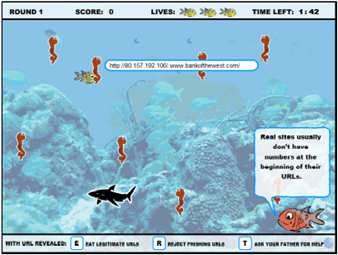
\includegraphics[width=0.9\linewidth]{images/antiphishingphil.png}   
    \caption{Anti-Phishing Phil game screen with the player fish interacting with a worm holding a URL, with the fish advisor giving advice to the player}
    \label{fig:antiphishingphil} 
\end{figure}

\subsection{What.Hack}
What.Hack \citep{wen2019hack} is a student project to create an anti-phishing training game in which players have to discern phishing emails from legitimate emails. The game takes the form of an (extremely simplified) email client. Once the user has made a choice, they must click either the accept or reject buttons based on their guess. For additional help the user can ask an in-game advisor to give hints, as show in Figure~\ref{fig:whathack_1}. On top of this, the players can access a ‘rulebook’, giving them a series of guidelines to follow to determine if an email is malicious. This application applies a much greater level of context to the simulated phishing attacks, from the actual design of the user experience right through to the content of the emails. 

Framing the game itself to take the form of an email client gives the player a greater frame of reference for what actual phishing attacks look like 'out in the wild'. However, the design of the client has been streamlined to the point of losing key elements of the contextual value of framing it as a email client. As shown in Figure~\ref{fig:whathack_2}, each of the emails contains 'Submit Phishing' and 'Allow Entry' buttons. For the regular phishing victim, these buttons do not exist within standard email clients and the 'gamification' of these elements only depreciates the important contextual value that a similar product might hold.

\begin{figure}[H]
    \centering
    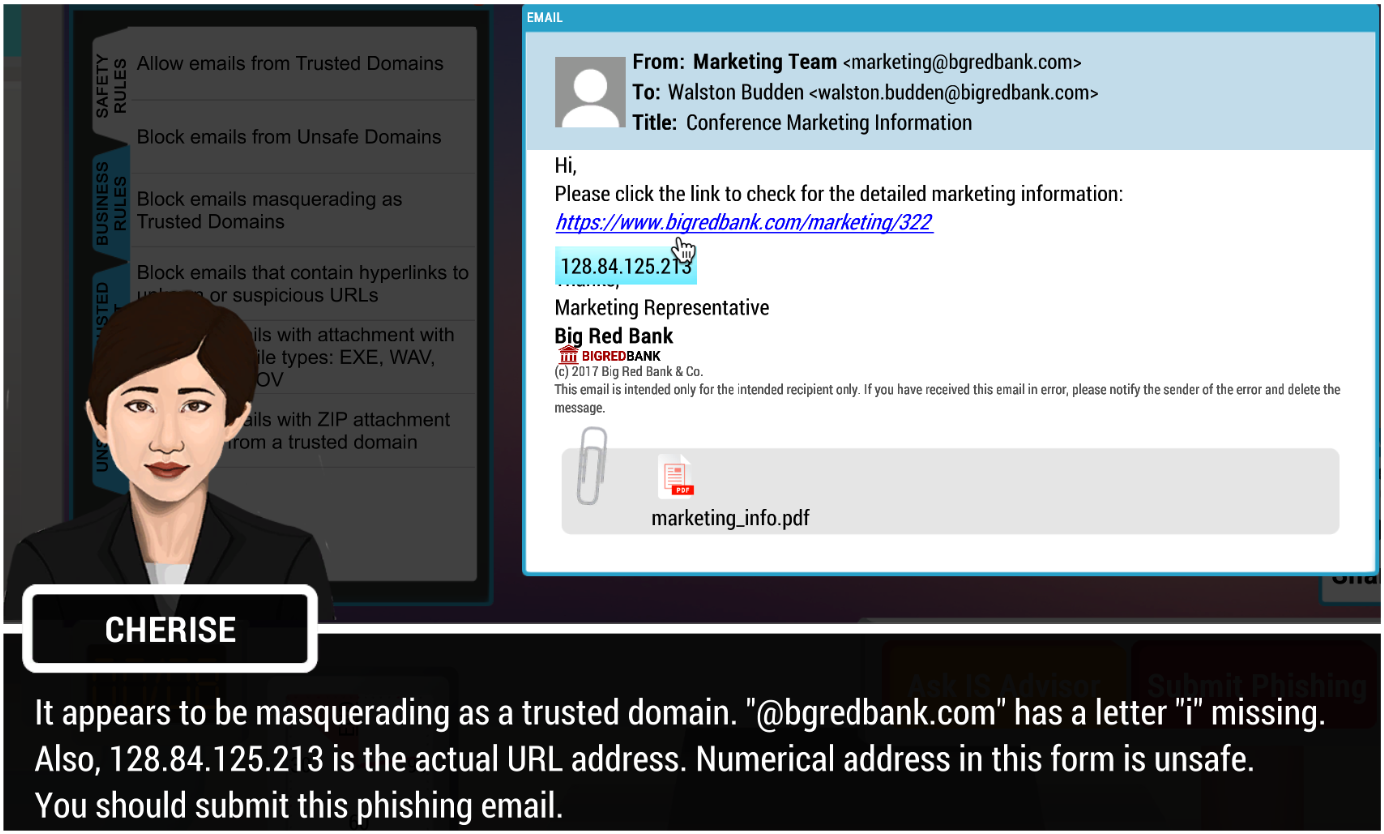
\includegraphics[width=1\linewidth]{images/whathack_1.png}    
    \caption{What.Hack main game screen with advisor giving player tips on the contents of the email, pointing out the use of typo-squatting and URL manipulation}
    \label{fig:whathack_1} 
\end{figure}

\begin{figure}[H]
    \centering
    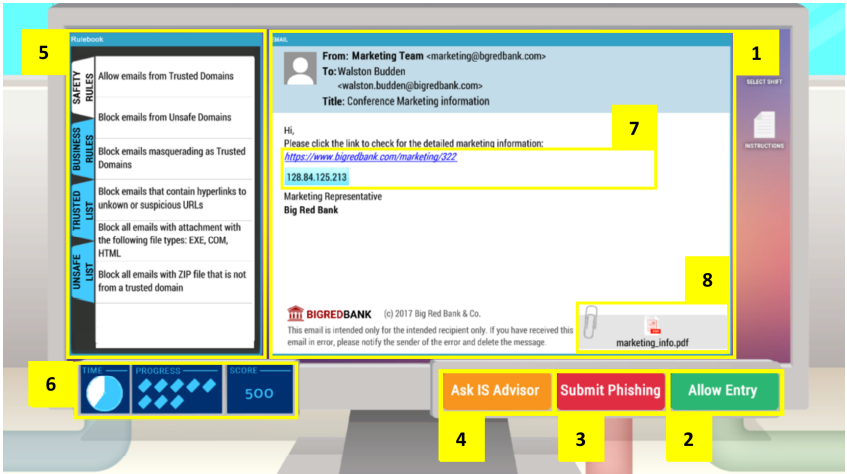
\includegraphics[width=1\linewidth]{images/whathack_2.png}    
    \caption{What.Hack main game screen with showing the buttons and available actions given to the player}
    \label{fig:whathack_2} 
\end{figure}

\subsection{PhishGuru}
PhishGuru \citep{kumaraguru2008lessons} was a training program used to train employees how to identify and avoid phishing attacks. The training scheme came in the form of an email which presented a short comic strip (Figure~\ref{fig:phishguru}) that briefly outlined the key red flags of a phishing email. Once this short phishing comic had been delivered to the participants, they were secretly sent fake phishing emails to their workplace email accounts by the creators of PhishGuru. These emails would collect data and statistics regarding how the participant would deal with the email. 

Although this training scheme makes use of similar advice and tips for avoiding phishing, implementing it through a comic strip makes poor use of any training techniques. The complete lack of contextual information or user interaction with the training material makes this an inadequate attempt at anti-phishing training. This is shown in the results in which only a very small difference between the control group and the group that received the training comic strip.

Despite this, the experiment to test the effectiveness of the training made excellent use of context. With each of the participant receiving a fake phishing email containing all of the phishing red flags, logging the actions made by the user when dealing with the email. The use of the participants actual email client under a blind test makes great use of ecological validity within phishing training. If this had been coupled with an improved initial training scheme, the validity and quality of the results would be much greater.

\begin{figure}[H]
    \centering
    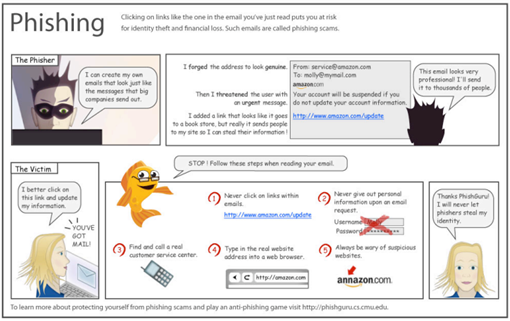
\includegraphics[width=1\linewidth]{images/phishguru.png}    
    \caption{The PhishGuru comic strip giving general tips to avoid phishing attacks }
    \label{fig:phishguru} 
\end{figure}

\subsection{Summary of Existing Systems}
Despite the similarities in objectives, all of these systems approach the training in very different ways. All of the systems teach the user similar phishing tactics such as typo-squatting and sound-squatting. However, in terms of context, most of the systems had poor context integration, often being too simplified (in the case of What.Hack) or virtually non-existent (PhishGuru). This shows a lack of understanding as to the best training methods when it comes to phishing, that being the importance of context for the user. 

The methods of evaluation for each of these systems differed, with the game-based training programs using the in-game score as a basis for the knowledge gained for the user, and the PhishGuru making use of contextual blind phishing test emails. Although the evaluation made by the PhishGuru project is excellent in terms of its similarity to real-world phishing attacks, the time required to implement a similar evaluation technique may be out of scope for this project. 

A table containing an overview of the different systems with a brief analysis can be seen in Figure~\ref{fig:sum_sys}.

\begin{table}[H]
\begin{adjustwidth}{-7em}{-5em}
\begin{tabular}{ | m{8em} | m{10em} | m{10em} | m{10em} | m{10em} | } 
 \hline
 \textbf{System} & \multicolumn{2}{l|}{\textbf{Phishing \& Context}} & \multicolumn{2}{l|}{\textbf{Quality of Training Methods}}  \\
 \hline
   & \textbf{Pros} & \textbf{Cons} & \textbf{Pros} & \textbf{Cons} \\
 \hline
  Anti-Phishing Phil & Links are similar to those found in phishing emails & lacks ecological validity  & Gives user an idea of how to spot red flags within URLs and hyperlinks & Difficult to apply to real life phishing attacks 
  \\
 \hline
 What.Hack & Accurate representation of real phishing attacks & Simplified and 'gamified' user experience takes away from validity & variety of knowledge gained and easily transferable to 'real world' applications & May not be difficult enough compared to real life spear-phishing attacks
  \\
 \hline
 PhishGuru & Gives reader a multitude of examples of how phishers can manipulate users & Information given on phishing and attacks is extremely brief and uninformative & Good for office work as can be kept near computer at all times & Very little actual content to training and user interaction
  \\
 \hline
\end{tabular}
\end{adjustwidth}
\caption{Brief summary of existing systems}
\label{fig:sum_sys}
\end{table}


%==================================================================================================================================
\chapter{Analysis/Requirements}

This chapter will detail the requirements of the project in MoSCoW format. These are taken from user stories and the research made, both of which have been informed by the chapter above.

\section{User Stories}
\textbf{Matt} is a bank manager and manages multiple teams within the department. Due to the rise in internet-based attacks, he wants to train his staff for the different types of attacks they may face, one of these being phishing attacks. Matt wants to give his staff regular anti-phishing training exercises that they can complete at work or at home. Due to workplace regulations and computer safety, he cannot install any software on the work computers so must have a training program that can run in a web browser. He wants to easily be able to see his employee's progress, including what they are consistently failing at and what their strengths are. 

\textbf{Thomas} is a team manager in the software development department for a large company. His team have plenty of technical experience and wish to keep up to date with the latest anti-phishing training techniques. He wants to be able to avoid the basic “tutorial” type training and go straight into the more technical, in-depth training. Thomas would be willing to install any type of training software as it would be easy for him to do. 

\textbf{Sophie} is an employee for the human resources department of a company. They have little to no technical experience outside of operating their email client and similar tasks. Due to recent phishing attacks, they have been instructed to learn about phishing and methods to prevent successful attacks. Due to their lack of experience, they need every aspect of phishing explained in detail for the training to work successfully. Due to the amount of emails she receives, she needs lots of varied examples of common signposts of phishing emails. Her lack of proficiency in technology means she requires something that does not need to be installed or have any complex set-up, preferably something she can use in her browser.

\section{Functional Requirements}
\subsection{Must Have}
\begin{tabular}{ | m{10em} | m{30em}| } 
  \hline
  \textbf{Requirement} & \textbf{Description} \\ 
  \hline
  Training & This application must train the user in anti-phishing practices as per the product description \\ 
  \hline
  Fail States & Effective training would entail the user must be able to pass or fail tasks based on their input \\ 
  \hline
  Context in Design & The application must make effective use of context within the look/feel of the application itself as well as the tasks given to the user \\  
  \hline
  Context in Content & The application must make use of different levels of context within the actual content of the exercises the user needs to perform \\  
  \hline
  Broad representation & This application must display a broad range of different types of phishing to the user, teaching them methods in detection and avoidance \\  
  \hline
\end{tabular}

\subsection{Should Have}
\begin{tabular}{ | m{10em} | m{30em}| } 
  \hline
  \textbf{Requirement} & \textbf{Description} \\ 
  \hline
  Reflection & The application should be able to report the user’s progress through the training, including their weakest and strongest points \\ 
  \hline
  Immersion & The user should find the application immersive in terms of familiarity and comfortability with the technologies they use on a regular basis \\ 
  \hline
  Assistance & The application should assist the user as much as possible without giving them the answer (if the user is struggling with the task) \\ 
  \hline
\end{tabular}

\subsection{Could Have}
\begin{tabular}{ | m{10em} | m{30em}| } 
  \hline
  \textbf{Requirement} & \textbf{Description} \\ 
  \hline
  Difficulty Customisation & The application could give the user control over how difficult the training tasks are to allow more technically advanced users to jump ahead to more advanced training techniques \\ 
  \hline
  Multiple "Campaigns" & The application could make use of a number of “real-life” phishing attacks as training exercises  \\ 
  \hline
  Glossary & The application could give the user access to a glossary containing technical terms with descriptions and/or examples \\ 
  \hline
\end{tabular}

\subsection{Would Be Nice To Have}
\begin{tabular}{ | m{10em} | m{30em}| } 
  \hline
  \textbf{Requirement} & \textbf{Description} \\ 
  \hline
  User History & The application would benefit from a form of training history for each user to view their progress over time \\ 
  \hline
\end{tabular}

\section{Non-Functional Requirements}
\begin{tabular}{ | m{10em} | m{30em}| } 
  \hline
  \textbf{Requirement} & \textbf{Description} \\ 
  \hline
  Ease of Installation & The application should be easy to install/use on a broad range of devices and environments (e.g. workplace, home PC, etc) \\ 
  \hline
  Multiple Devices & The application should work across a broad range on devices including tablets and mobile phones \\ 
  \hline
  Accessibility & The application should train people at any knowledge level and level of technical skill \\ 
  \hline
  Speed & The application should be fast to boot and operate \\ 
  \hline
\end{tabular} 

%==================================================================================================================================
\chapter{Design}

This chapter details the process of designing all aspects of this application, including system architecture, design of training materials, and wireframes.

\section{Initial System Architecture}
As an initial design step, a system diagram needs to be created. As you can see below, the system architecture diagram is a three-tier diagram for each of the key elements of the application: client tier, logic tier, and database tier \citep{aarsten1996patterns}. 

\begin{figure}[H]
    \centering
    \frame{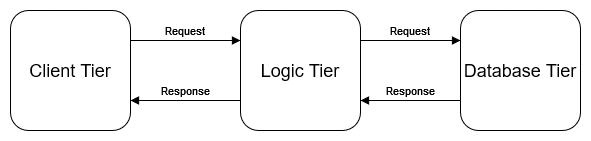
\includegraphics[width=0.9\linewidth]{images/initial_arch.png}}  
    \caption{Initial system architecture outlining basic interactions between core systems}
    \label{fig:initial_arch} 
\end{figure}

The client tier of the diagram gives an overview of the user interface of the application, including the different pages the user can view. The logic tier details the application backend interface or general logic. The database tier details the location of all relevant application data storage.
\newline

Between each of the tiers, there are indicators of incoming and outgoing communication between the tiers. With the client tier communication is exclusively with the logic tier, and the logic tier interaction is with both the client tier and the database tier. At no point does the database tier interact directly with the client tier.
\newline

The three-tier model was appropriate for this project due to the scalability and reliability of its fundamental design. Each tier is independent enough to be scaled as needed without too much impact on the other tiers. In addition, if a single tier starts underperforming or fails, the other tiers will not be impacted by this and continue to operate. All of this leads to a more efficient and faster development time.

\section{Training as a Game}
Effective training requires a greater level of user interaction which is interlinked with an environment which simulates a real life attack. A fully embedded training scheme would be out of scope for this project but a simulated environment with fake emails and phishing attacks would be the best solution. A training game is the logical extension of this, similar to the What.Hack and Anti-Phishing Phil training games, but would attempt to improve on the existing systems. The mechanics of the game would have to abide by a strict rule of contextual awareness whereby it would treat itself as a standard email client with little to no reference to the simulation or make use of gamified terminology (such as "Levels" or "Points").

\section{Context in Design}
The user interface for this training game must take into account key usability heuristics \citep{nielsen2005ten}. These heuristics cover a variety of principles concerning the design of user interfaces, but there are several which play a larger part in this project, namely the second and sixth heuristics. The second principle states there should be a match between the system design and the world of the user, that which they inherently understand. This is key in the application of context and ecological validity in terms of the transfer of learnt knowledge from the training being easily applicable to a real phishing attack. The sixth principle promotes the concept of users being able to intuitively navigate and access the program with minimal (or no) instructions. This gives the user autonomy in moving up a level or replaying sections of the game.

The design of the application is key to immersing the user into an accurate simulation of a phishing attack, this being an email client. There are numerous email clients on the market, the most popular being Google Mail, Microsoft Outlook, and Apple Mail \citep{emailclientlitmus}. For the Apple and Outlook clients, a similar approach in design is taken, with the list of emails on the right hand side and the full selected email display on the left. With the Google Mail client, the email list is more vertically condensed per email but takes up the entire page. Once an email is clicked, the selected email will take up the whole page. Above these sections is a navigation bar which gives contextual options to the user (often related to the selected email). 

For this application, I will attempt to combine components of the Apple Mail (Figure~\ref{fig:applemail}) and Outlook (Figure~\ref{fig:outlook}) clients as these give great overall visibility for emails. From the possible options, Microsoft Outlook was chosen as the base design of the application. This was mainly chosen due to a higher level of experience with Outlook over the other possible clients. This design will effect the colour scheme and layout of outlook.

This context should also apply to the game mechanics themselves. In this sense, the player/user would simply operate the email client as they would a normal client. Therefore 'gamified' terms will not be used in the actual content of the application, for example incrementing the levels will not be displayed to the user as a "next level" button. Instead making use of terms that would make sense in the context of a workplace email client such as "get mail". This will not only allow users to easily make use of the game but also have a more effective integration with real phishing attacks.

\section{Level Progression}
Being a game, level progression is a key element of the design process. If the training features work as intended, each level should layer new (and increasingly difficult) phishing techniques. This process of gradually introducing phishing techniques should effectively build up a knowledge base for the user to apply to real world phishing attacks. Each level has a planned feature to be implemented, as shown below:
\begin{itemize}
    \item Level One: Very obvious attempts at phishing attacks with clearly suspicious email content
    \item Level Two: Phishing emails begin to use links while becoming slightly more inconspicuous 
    \item Level Three: Phishing emails make use of both links and attachments with relevant workplace email content
    \item Level Four: Phishing emails become very difficult to detect by impersonating other members of staff and departments (the authors of previous non-phishing emails) while also using links and attachments
\end{itemize}


\section{Wireframes and Features}
There are several main views within the core design: the login view, the main email view without email displayed, and the main email view with an email displayed. Wireframes were created for each of these views in order to hone a standardised design pattern. The design of all of these screens will be in the format of an email, for the sake of user immersion and ecological validity. This includes content that could be considered immersion "breaking", such as the results screen. The user will never encounter an email like this in the real world but the consistency of this design is paramount for the training to be effective. 


\subsection{Main View}
This is the main view that the users will spend the majority of their time navigating. In this screen, users will have a series of emails arrive, where they need to review/analyse each email to determine whether the email is a phishing attack or not. For each of the emails, the user will have a choice as to whether they should accept the email (if the user deems it as non-malicious) or if they should reject it (if the user considers it to be a phishing email). Once all of the emails in the selection have been either accepted or rejected, the user is given the option to review their decisions and progress to the next set of emails. Each email will contain text similar to those found in regular workplace emails, occasionally sporting attachments and links. However, for each of these groups of emails, several will be phishing emails, making use of the numerous phishing tactics.

\begin{figure}[H]
    \centering
    \frame{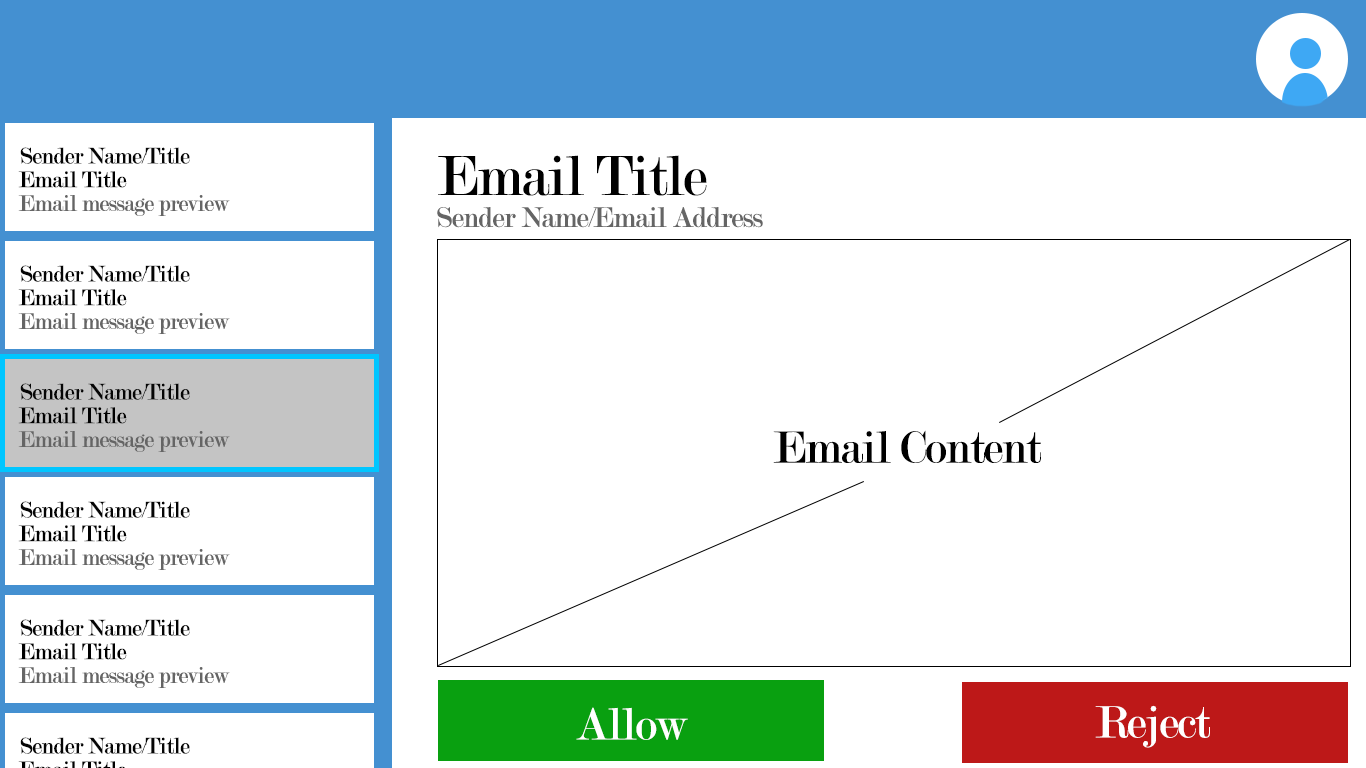
\includegraphics[width=1\linewidth]{images/main_screen_wf.png}}
    \caption{Wireframe of the main play screen}
    \label{fig:main_wf} 
\end{figure}

\subsection{Results View}
Giving feedback is an important part of training because it provides the user with the opportunity to review their progress. On this screen, the user will be presented with the number of correctly identified emails (rejected phishing emails and allowed non-phishing emails) and incorrect guesses. There is also a breakdown of the incorrect guesses, that being the number of false positives (accepting phishing emails) and false negatives (rejecting non-phishing emails). From this screen, the user has two options: continue to the next level or repeat the current level in order to correct their mistakes. 

\begin{figure}[H]
    \centering
    \frame{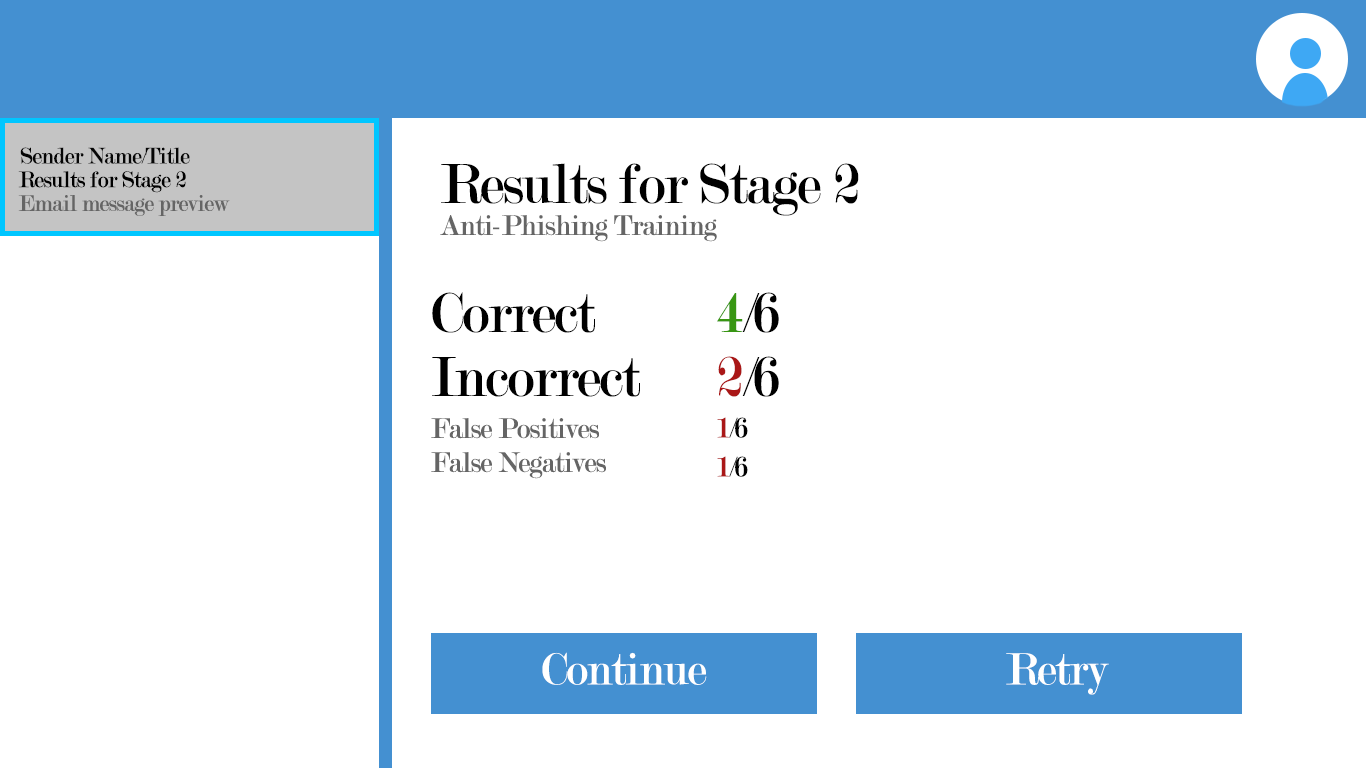
\includegraphics[width=1\linewidth]{images/results_wf.png}}
    \caption{Wireframe of the end of level results screen}
    \label{fig:results_wf} 
\end{figure}

\subsection{Menus \& Additional Views}
The main menu (as shown in Figure~\ref{fig:menu_wf}) will provide the user with numerous options for both new and returning users. New users will be prompted to take the tutorial which will guide the user on how to "play" the training game and key aspects of the interface. For each of the levels there will be a button to instantly start the game at the specified level.

\begin{figure}[H]
    \centering
    \frame{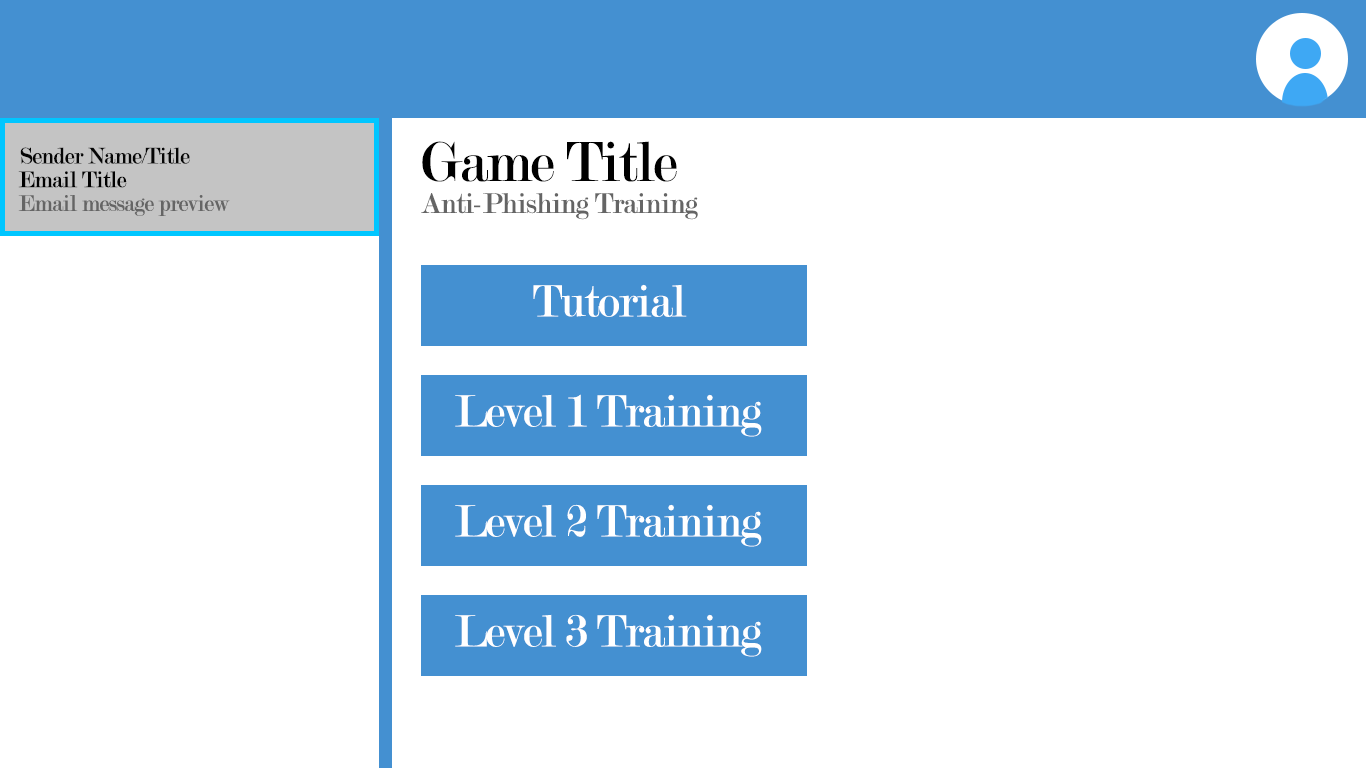
\includegraphics[width=1\linewidth]{images/menu_wf.png}}
    \caption{Wireframe of main menu screen}
    \label{fig:menu_wf} 
\end{figure}

%==================================================================================================================================
\chapter{Implementation}

This chapter outlines the process of development and implementation of the application, adhering to the design specifications put forward in the previous chapter.

\section{Application Base}
As a result of the decision to emulate Microsoft's Outlook email client, the obvious choice for development/design would be a web-based application. This not only fulfills the requirements set out by the user stories in terms of ease of installation and accessibility from multiple device types, but also adheres to the core philosophy of emulating an environment in which phishing attacks occur (a web based email client).

\section{Technologies}
 A three tier architecture is suited for this project, as outlined in the design section. See Figure~\ref{fig:tech_arch} for an updated architecture diagram that includes the technologies used in the application.

\begin{figure}[H]
    \centering
    \frame{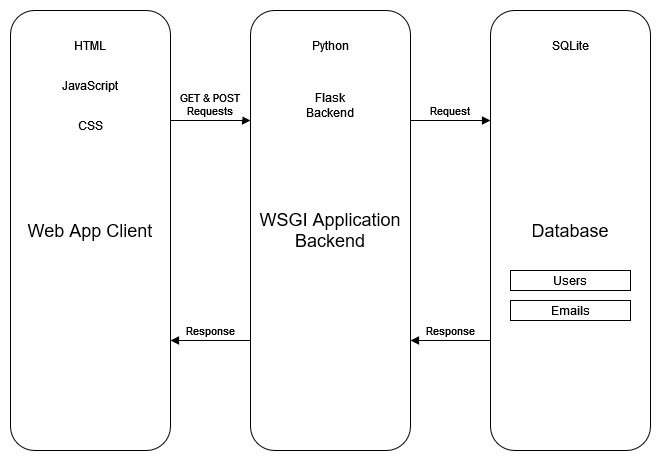
\includegraphics[width=0.9\linewidth]{images/tech_arch.png}}  
    \caption{Updated system architecture outlining technologies used in core systems}
    \label{fig:tech_arch} 
\end{figure}

\subsection{HTML, CSS, & JavaScript}
The client tier is the web application itself, making use of HTML, CSS, and JavaScript to display the pseudo-email client to the user. The pages simulate the basic design and functionality of outlook, as shown by the wireframes. The JavaScript gives some basic logic to the functionality of the game, such as scoring and transitioning between level states. JavaScript is also the primary method in which emails are retrieved from the database of emails.

\subsection{Flask}
In the planning stages of developing the application back-end, a choice needed to be made between the two popular Python web frameworks: Django and Flask. Despite prior experience with Django, Flask was chosen due to the lightweight nature of the framework. Django is packaged with numerous tools and scripts which is useful in the majority of web-based applications. However for this project only a lightweight microframework is required and, if necessary, extensions to this framework can be added from a large library of supported extensions. 

Flask makes use of the Application Factory Design Pattern \citep{flask}. This is the process of instantiating a class and then using objects as separate modules to that base class. In the case of this project, the Flask application is instantiated in the \verb| __init__.py| file and registers all modules (named blueprints) that are used in the application. These blueprints are modular, making use of templates and views to generate the different pages used within the project. The two blueprints created for this project are:

\begin{itemize}
  \item \textbf{Authentication}: This is the page in which users will be able to register and login to their accounts, the details of which are stored in a database. All of the passwords are safely stored and hashed using the Flask API \verb|werkzeug.security| functionality \citep{werkzeugSecurity}. This also checks against the database if the user already has an account under the username so multiple accounts of the same name cannot be created. If the user is not logged in they will be unable to access any of the content of the application.
  \item \textbf{Email}: This is the page which simulates the main functionality of the email client, with emails being viewable, allowing the user to perform various actions on those emails.
\end{itemize}

Due to the modular nature of Flask and the blueprint systems, it is extremely simple to extend the functionality of the application and create new views/pages.

Each of the blueprints contain their own callable functions that can be called by JavaScript and HTML. For instance, the JavaScript will make a HTTP request to the email blueprint in order to execute the relevant SQL query, returning the emails needed for the current level.

The code used to create the training game and all blueprints can be seen in Listing~\ref{lst:blueprints}, showing the modularity of this design.

\begin{lstlisting}[H, language=python, caption={Creation of training app and all associated blueprints in the \_\_init\_\_.py file}, label=lst:blueprints]
    def create_app(test_config=None):
    	app = Flask(__name__, instance_relative_config=True)
    	
        ...
    
    	app.register_blueprint(auth.bp)
    	app.register_blueprint(email.bp)
    	app.add_url_rule('/', endpoint='email')
    
    	return app
\end{lstlisting}

\subsection{SQLite}
SQLite is a lightweight version of the SQL database engine. Due to the low requirements and faster data retrieval/storage, it is often used for basic databases within webapps. However, this functionality is limited with no support for concurrent changes to the database or multiple database-user types (e.g. admin and viewer access to database). It has inbuilt integration with the Flask WSGI and so was easy to implement using the \verb|sqlite3| package. The database requirements for this project simply needed a method to store a collection of emails and basic userdata, therefore SQLite was perfect. Many of the drawbacks of using SQLite were inconsequential as the specifications of this webapp did not require the missing features.

The structure of the database consists of two tables: \textit{Users} and \textit{Emails}. The \textit{Users} table only required three fields: ID, username, & password (hashed).

The \textit{Emails} table stores all the emails that will be sent to the user through the duration of the training game. It contains seven fields: ID, difficulty (level in which the email appears), author, header, datetime, phishing (boolean bit indicating if the email is a phishing email), & content (main body of the email). Both of these can be seen in Figure~\ref{fig:database}. 

\begin{figure}[H]
    \centering
    \frame{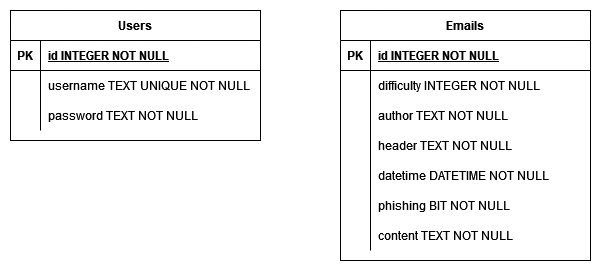
\includegraphics[width=0.9\linewidth]{images/database.png}}  
    \caption{Database ER Diagram (despite no relations between the tables)}
    \label{fig:database} 
\end{figure}


\subsection{Python Anywhere}
In order to distribute the web application for user evaluations, it was hosted on PythonAnywhere. This allows web frameworks, such as flask, to make use of cloud computing and storage. This required partial modification to the Python script in order to successfully host the application online, including configuration of a WSGI file. The ease of integration and distribution greatly assisted in the evaluation process.

\subsection{GitLab and Version Control}
The codebase of this project was stored and maintained using GitLab and several backups. Version control is extremely important in breakdown and simplifying the development process through features such as branching and merging \citep{otte2009version}. Branching was used when implementing new features, keeping the master branch stable and functional. Once the feature branch has been completed and debugged, it is merged with the master branch. This also implements semantic versioning to label the new features and patches added to the codebase \citep{prestonwerner_2022}.

\section{Functionality}

\subsection{User Authentication}
These pages include a registration page (Figure~\ref{fig:registration_page}) and a log in page (Figure~\ref{fig:log_in_page}). The registration page simply takes two user inputs: a username and password. The usernames are checked against the database to see if the account already exists; if so, an error message is displayed to the user at the top of the form. Otherwise a new entry is created in the database for that user.

The log in page is very similar in design to the registration page, also taking the username and password as inputs. The user must have previously registered to successfully log in and access the rest of the training game. Errors, such as an incorrect password or unregistered user, are also displayed through an error message at the top of the form.

The flask authentication process is used in both sections to check for existing users within the database. If an existing user is found upon registration, then an error is returned. When logging in, the database of users is searched for an existing user of the same username (which must be unique) and, if found, the entered password is checked alongside the hashed password stored within the database. If this is accepted, then the user is successfully logged in, otherwise returning an error. These registration authentication checks can be seen in Listing~\ref{lst:flask_auth}.

\begin{lstlisting}[H, language=python, caption={Registration authentication checks in the auth.py file}, label=lst:flask_auth]
    if error is None:
		try:
			db.execute("INSERT INTO user (username, password) VALUES (?, ?)",
			(username, generate_password_hash(password)),
			)
			db.commit()
		except db.IntegrityError:
			error = f"User '{username}' is already registered"
	else:
		return redirect(url_for("auth.login"))
	flash(error)
\end{lstlisting}

\subsection{Level Introduction Stage}
At the beginning of each level, a short introduction email is received hinting at the basic concepts to be introduced within that level. This will also acclimate the user to many of the terms and tactics associated with phishing. The level one introduction email explains the basics of email safety as well as a short tutorial on how to navigate the web app. The second introduction email gives more advice to the user on interacting with links and phishing tactics to be aware of (namely typo-squatting and sound-squatting). The third introduction email advises the user on dealing with potentially malicious email attachments, giving tips on what to look at when inspecting attachments. The fourth and final introduction email tells the user that there has been a data breach within the company and that employee records have been stolen. This means that the user can no longer trust emails from other departments or fellow colleagues and must use all the training they have received in the previous levels to correctly identify the phishing emails.

\subsection{Main Level Stage}
Each of the levels consist of the player assessing a number of emails to delete or report those of which are assessed as phishing. Each level contains 10 emails each with increasing numbers of phishing emails. Each email has been modified from real workplace emails, with changes made to protect privacy and other data. The phishing emails have also been adapted from real world phishing emails in order to maintain the integrity and consistency of the training with genuine phishing attacks. Each email displays a read and unread indictator similar to that found in the Outlook email client (shown in Figure~\ref{fig:read_unread}). Once the emails have been read, the "Commit Report" button becomes available to click, sending the user into the summary stage of the level. If the user thinks they have detected a phishing email, they have two options in dealing with it. They can either report the email as phishing or simply delete the email. Genuine email clients contain a multitude of options and tools when dealing with emails and so the training game must (at least partially) reflect this. One such tool is the \textit{Contacts} button which will display a list of the in-game work colleagues the player is expected to receive emails from. The user can use this to establish a baseline of more trustworthy emails/senders. However, this will be tested as the user progresses to the more difficult levels.

\begin{figure}[H]
    \centering
    \frame{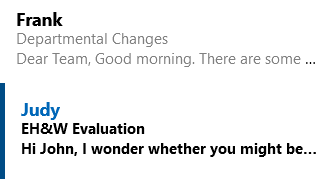
\includegraphics[width=0.6\linewidth]{images/read_unread.png}}
    \caption{Emails displaying the read status (top) and unread status (bottom)}
    \label{fig:read_unread}
\end{figure}

The levels introduce a series of phishing techniques gradually, with each level becoming increasingly difficult. Context is also gradually introduced with the initial levels containing easily detectable, contextless emails. These do not contain any information relevant to the workplace or to the user themselves. Although these are often picked up by spam detection, providing the player an initial frame of reference for detecting "easy" phishing emails is key to layering on more difficult phishing tactics. 

Level one contains only two phishing emails, both of which contain obvious fraud attempts and requests for finances. One of the phishing emails also includes a clearly suspicious hyperlink (e.g. \textit{http://www.86986568.com.cancercharity.9876875876987.aoseiuvnbsoiven.ru/oiuhaocin}), introducing the idea that hyperlinks can be very dangerous and are often used in phishing attacks. 

The second level builds on the use of links within phishing emails, along with the tactics used in obscuring these links. Three phishing emails are present, each using a different technique. One email makes use of legitimate companies and details within the hyperlink in an, albeit poor, attempt to legitimise this link (e.g.  \textit{http://364.974.25.089:64/mcafee.com/virusprotect.html}). This level also introduces the concept of typo-squatting, changing some of the letters within a URL to trick the user into thinking it is legitimate (e.g. \textit{http://www.anazon.com/accountsecurity}). The final technique used in this level is link obfuscation whereby the hyperlink itself is hidden in text and the user must hover over the link in order to reveal the destination (e.g. \textit{\underline{Check Account} reveals https://247.972.76.314:76 as the URL}). These emails are more focused on context than the previous level but still lack any real information relating to the user or the company, instead basing the malicious emails on those one \emph{might} receive on a workplace email address. 

Level 3 contains 4 phishing emails, making use of both links and file attachments. Attachments can be used in phishing attacks to install malware, spyware, and data extraction software, so assessing these is a core principle in anti-phishing training. On top of this, file attachments to emails are commonplace in an office work environment (which is reflected in the non-phishing emails in this level), making the detection of phishing emails more difficult for the user. The phishing emails in this level make use of a number of attachments, namely, \textit{.pdf} files, \textit{.exe} applications, and \textit{.html} files. Excluding the \textit{.exe} file, these file types are used by both phishing and non-phishing emails, so the user must analyse the content of the email in the context of the rest of the emails to assess how malicious each email is. A workplace context is introduced into the phishing emails, making reference to common concepts in an office environment, including training and invoices. The URL techniques from the previous level are also included among emails of all types in this level.

The final level contains an even split of 5 phishing emails and 5 non-phishing emails. These phishing emails are the most difficult to detect as some impersonate other members of staff and other departments within the business. As a result of this, the user will have to closely analyse the content of each email, along with any links or attachments they may contain, to succeed in this level. Many of the attachments within the phishing emails have been disguised as official-looking documents from legitimate sources with only a few indicators (such as file size or prior context) revealing their enmity. One of the key sections of this level are the two emails from the same employee, one being a phishing email impersonating a real employee. The second email from this employee references having their email account details stolen and emails being sent out without their knowledge. The user must link this with the previous email (containing an attachment) in order to correctly report it as phishing.

\subsection{Level Summary Stage}
At the end of each level, once the user has clicked the "Commit Report" button, they are greeted by a new set of emails. The first email is the summary of the users performance for that level, detailing the total number of phishing and non-phishing emails alongside how many emails the user reported, deleted, or ignored. This summary also shows how many phishing emails the user ignored and failed to take action on. The following emails are either the phishing emails that were ignored or the non-phishing emails that were incorrectly reported. This stage is critical in user training, giving the user an insight into any errors they may have made and how to avoid this mistake in the future. On top of this, a basic scoring system has been implemented giving the user points based on the number of correct guesses and penalised for the number of mistakes made. 

\section{Changes Made}
From the previous wireframes and design choices, some changes have been made to the functionality and design of the program.

\begin{itemize}
  \item \verb|Main Menu|: this has been implemented almost exactly as shown in the wireframe (Figure~\ref{fig:menu_wf}) and can be seen in Figure~\ref{fig:menu_final}.
  \item \verb|Email Screen/Main View|: The main design of this screen is similar to the wireframe, with several additions, namely, the additional navigation bar which gives the user email specific actions depending on the content of the display. Three buttons are permanent fixtures on the left-hand side: \textit{"Get Mail"} which (once all emails have been read) allows the user to progress to the next stage of the level, \textit{"Commit Report"} which (once the emails have been read) allows the user to submit their decision and progress from the main stage to the summary stage, and the \textit{"Contacts"} button which displays the list of work colleagues within the "office". This screen has been split into two sections, outlined in the following points:
    \begin{itemize}
        \item \verb|Intro Screen|: This screen contains a single email detailing the key flags that the user should be looking out for when detecting phishing emails. This is done in an immersive way as to not break the context of the game, and so is displayed as a daily email from the player's boss. This can be seen in Figure~\ref{fig:intro_final}.
        \item \verb|Level Screen|:This screen contains the main contents of the level, that being the list of emails in which the player has to detect phishing. In the original design, the decision to either \textit{"allow"} or \textit{"reject"} an email was used, however this broke the core design rule that had been established: to keep the training simulation as close to a real life scenario as possible, retaining all context and immersion where possible. As a result, this was altered to fit in line with the outlook design, that being an additional set of buttons on the newly created navigation bar. These buttons will only appear when an email is displayed in full view, giving the user the option to either delete the email or report the email as phishing. For this, the "report as phishing" function was weighted higher (giving +2 points per correct report) than deleting the phishing email (+1 point per correct deletion). The reason for this being that reporting an email as phishing will not only prevent the phishing attack from working but will also highlight this in any phishing detection or auto-deletion system. The screen can be seen in Figure~\ref{fig:email_final}
    \end{itemize}
  \item \verb|Summary Screen|: This screen is also similar to the wireframe although more information is displayed. The summary now includes the total number of emails in the level, the number of emails the user has reported as phishing (including the number of correctly report phishing emails), the number of emails that have been deleted (along with the number of phishing emails deleted), the number of phishing emails not reported or deleted, and the number of non-phishing emails reported as phishing. The cumulative score of the user is also displayed at the bottom of this screen. Alongside this, the phishing emails that were not caught by the user (or the non-phishing emails that were incorrectly reported) are now displayed as separate emails on the left-hand side, allowing the user to view them to re-assess the decisions they made. This screen can be seen in Figure~\ref{fig:summary_final}.
\end{itemize}

\section{Challenges Faced}
Throughout the development of this application, a number of challenges were faced. Towards the end of the development cycles, research was performed on single-page web applications (SPA). This research concluded that AngularJS may have been better suited to the development of such an application \citep{jadhav2015single}. Single-page applications are web-based applications that base all content around a fixed, one-page view with dynamically updated data. Although a form of this has essentially been implemented in the current web application using standard JavaScript and CSS, AngularJS tackles this problem much more efficiently. The current state of the JavaScript code is fairly disorganised and difficult to fully understand, as many compromises had to be made to effectively implement this SPA. Unfortunately, due to development time constraints and lack of developer experience in AngularJS, the project could not be retrofitted to make use of this technology. With more development time, reimplementing this web application with an AngularJS framework would be of great benefit to the clarity and efficiency of this application and the codebase.

As previously mentioned, during the design phase, the initial plan was to implement \textit{Accept} and \textit{Reject} buttons at the bottom of each of the emails for the user to assess which of the emails was a phishing attack. However, this created a dissonance between the context-based approach of the application with the actions the user would perform. After analysing this, a solution was found through the creation of the \textit{Delete} and \text{Report as Phishing} buttons. These can often be seen in applications such as Outlook (Figure~\ref{fig:outlook_report} and so adhere to the requirement for immersion and context. As a result of this, the \textit{Accept} button was removed entirely as the "acceptance" of an email is simply to not take an action that would remove that email from the inbox.





%==================================================================================================================================
\chapter{Evaluation} 

This chapter outlines the testing and evaluation performed on the application and the training materials.

\section{Unit Testing}
Unit testing was performed on the application to ensure all aspects of the interface were working correctly and gave expected results. This testing is often know as black box testing and white box testing. Black box testing is used to test all facets of the front-end and user interface whereas white box testing is used to investigate the functionality of the back-end (out of view of the user) to ensure all calculations and methods are performing correctly. Table~\ref{table:black_box} shows the black box tests performed on the application followed by the expected result and the actual result of the test. Table~\ref{table:white_box} shows the white box tests performed on the application in the same format.
\begin{table}[H]
\begin{tabular}{ | m{10em} | m{20em}| m{10em} | } 
  \hline
  \textbf{Test} & \textbf{Expected Result} & \textbf{Result of Test} \\ 
  \hline
  Registration & User can register an account & as expected \\ 
  \hline
  Registration Validation & User cannot register two accounts with the same username & as expected \\ 
  \hline
  Log in & User can log in with a registered account & as expected \\ 
  \hline
  Log in Validation & User cannot log in with a non-registered account & as expected \\ 
  \hline
  Menu Display & User is presented with the main menu after successfully logging in & as expected \\ 
  \hline
  Reporting and Deleting Emails & User can tag emails to report or delete & as expected \\ 
  \hline
  Reporting and Deleting Validation & User can only either report or delete a single email & as expected \\ 
  \hline
  Stage Transition & User can only progress to the next stage (using the commit report button) after reading all emails & as expected \\ 
  \hline
  User Scoring & User points are displayed correctly & as expected \\ 
  \hline
  Level Transition & User can transition to the correct level & as expected \\ 
  \hline
  Level Selection & User can jump to the correct level from the main menu & as expected \\ 
  \hline
\end{tabular}
\caption{Black box tests with expected outcomes and results}
\label{table:black_box}
\end{table}

\begin{table}[H]
\begin{tabular}{ | m{10em} | m{20em}| m{10em} | } 
  \hline
  \textbf{Test} & \textbf{Expected Result} & \textbf{Result of Test} \\ 
  \hline
  Registration & After registration the database stores the user account & as expected \\ 
  \hline
  Account Retrieval & the database returns the correct user information after log in & as expected \\ 
  \hline
  Email Retrieval & The database returns the correct selection of emails based on the level & as expected \\ 
  \hline
  Scoring Calculations & the JavaScript correctly calculates the user score for each level & as expected \\ 
  \hline
\end{tabular}
\caption{White box tests with expected outcomes and results}
\label{table:white_box}
\end{table}

As shown by the results above, all testing returned expected results. Any bugs that were found were fixed upon discovery during implementation.

\section{User Evaluation}
The evaluation process required an assessment of the training material itself and the application as a training tool. For this, a user evaluation was created, testing the material on users of varied technological ability and knowledge. A form was created to be given before and after the participants used the application in order to compare the level of phishing training and knowledge gained through its use. The form itself was distributed through Google Forms, requiring the participant to reflect on their existing knowledge of phishing and related cyber-attacks (the questions can be seen from Figure~\ref{fig:ques_1} onwards). The questionnaire was split into three sections: participant background, statement agreement, and phishing knowledge. The participant background section asks the participant a series of questions regarding their experience with technology and phishing. The phishing statement agreement proposes a series of statements regarding the technology used by the participants along with security software they may use, the participant must then respond with their levels of agreement (strongly agree to strongly disagree). The final section of the questionnaire tests the participant on their current knowledge of phishing and phishing strategies. Once the participant has completed the survey, an observed run exercise was held using the training web application. Once completed the user score was recorded and the participant was asked to complete the questionnaire again using the knowledge they may have gained from the training. The ethics checklist was completed by all participants prior to performing the questionnaire (Figure~\ref{fig:ethics}).

\subsection{User Evaluation Results}
In this section, the results of both the training game and the questionnaire (before and after playing) are analysed to reveal the quality of the training application. 

With the initial results of the test section of the first questionnaire (pre-training), users scored on average 4.57 out of a total of 8 marks. The majority of users had previous experience with technology and some basic form of cyber-security, which may be as a result of the lack of disparity with the age ranges of the participants as 83\% were between the ages of 21-30 (Figure~\ref{fig:part_age_range}). For most participants, this experience resulted in the majority of the test questions being correctly answered. However, the question regarding the detection of secure websites had a 0\% success rate, with the majority of participants believing that a "padlock appearing on the URL" would be enough to deem the website secure, despite evidence pointing otherwise \citep{spadafora_2018}. On top of this, around half the participants believed that an email using a button to redirect you to a webpage had no discernible method of viewing the link without initially clicking on it.

\begin{figure}[H]
    \centering
    \frame{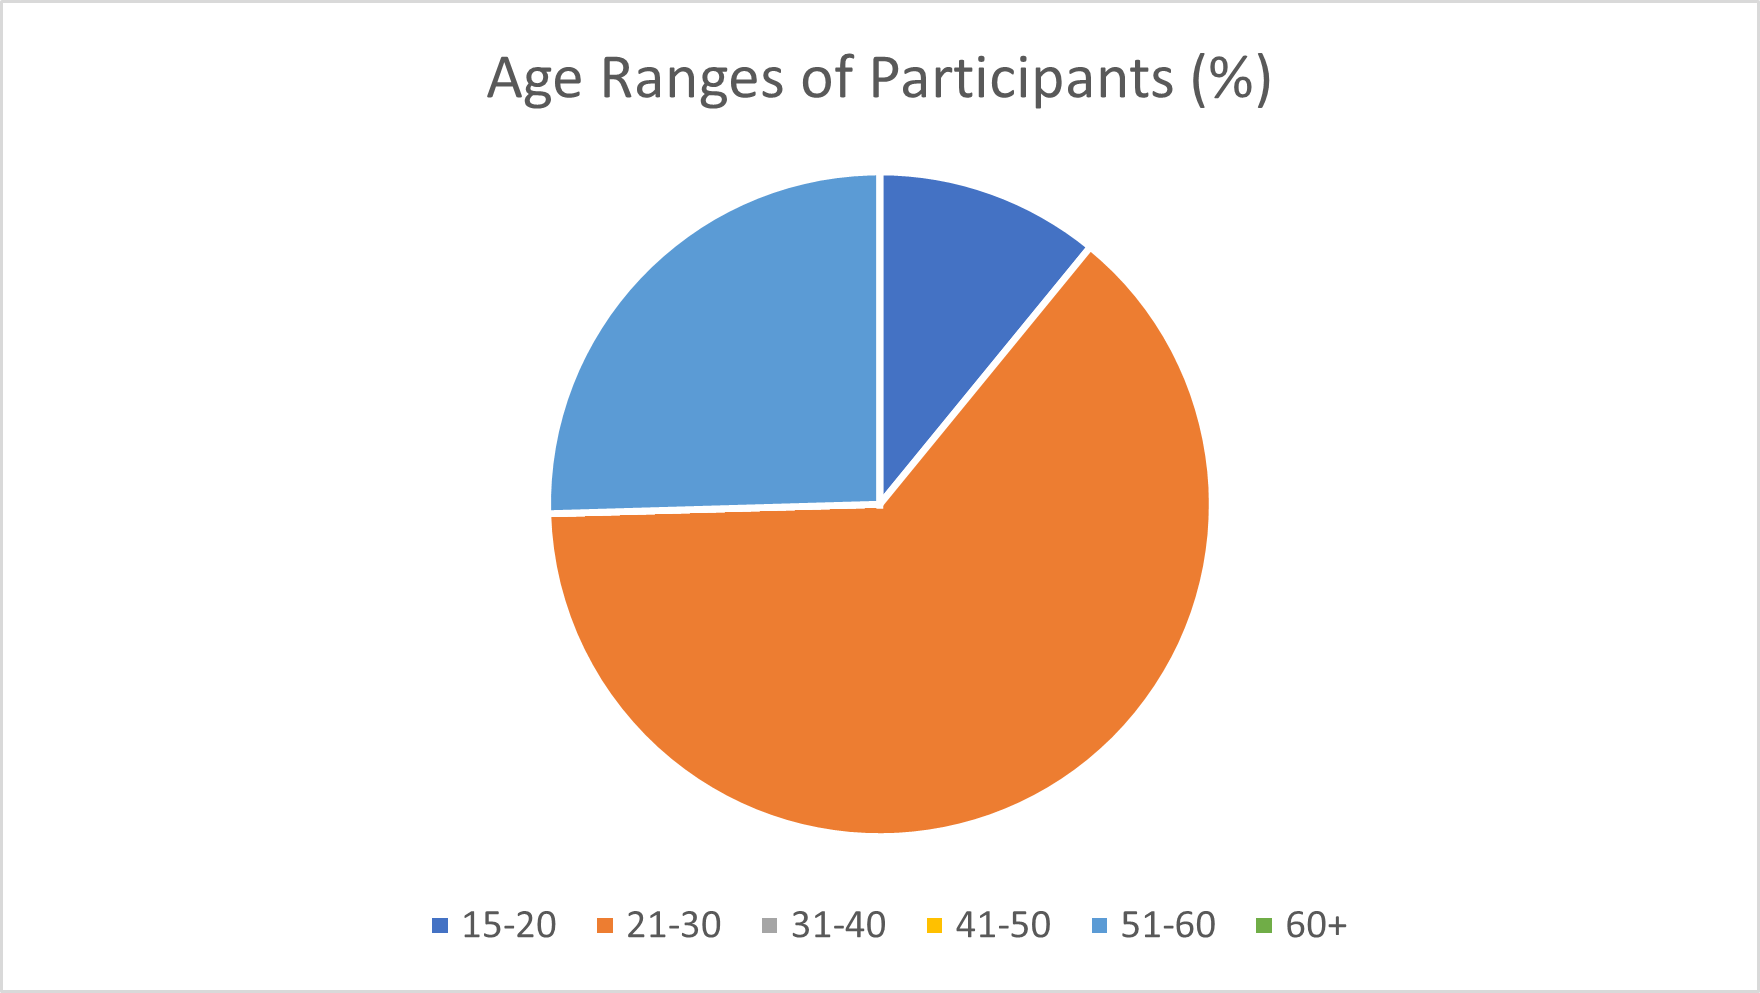
\includegraphics[width=1\linewidth]{images/part_age_range.png}}
    \caption{Age ranges of participants used in evaluation}
    \label{fig:part_age_range}
\end{figure}

During the training, participants were asked to complete the training game while being observed by the developer. The observer could not assist the participant in any way and could only record the results of the participant's score. The maximum score a participant could reach was a total of 28 points, given that they correctly reported all phishing emails as phishing without mistakes. Figure~\ref{fig:training_score} shows the final score for each of the participants, with an average final score of 24 points. This average is surprisingly high, especially when compared to the score of the questionnaire (compared in Figure~\ref{fig:score_comp}). This shows that the difficulty of the training application may have been too low for those with experience in technology and security.

\begin{figure}[H]
    \centering
    \frame{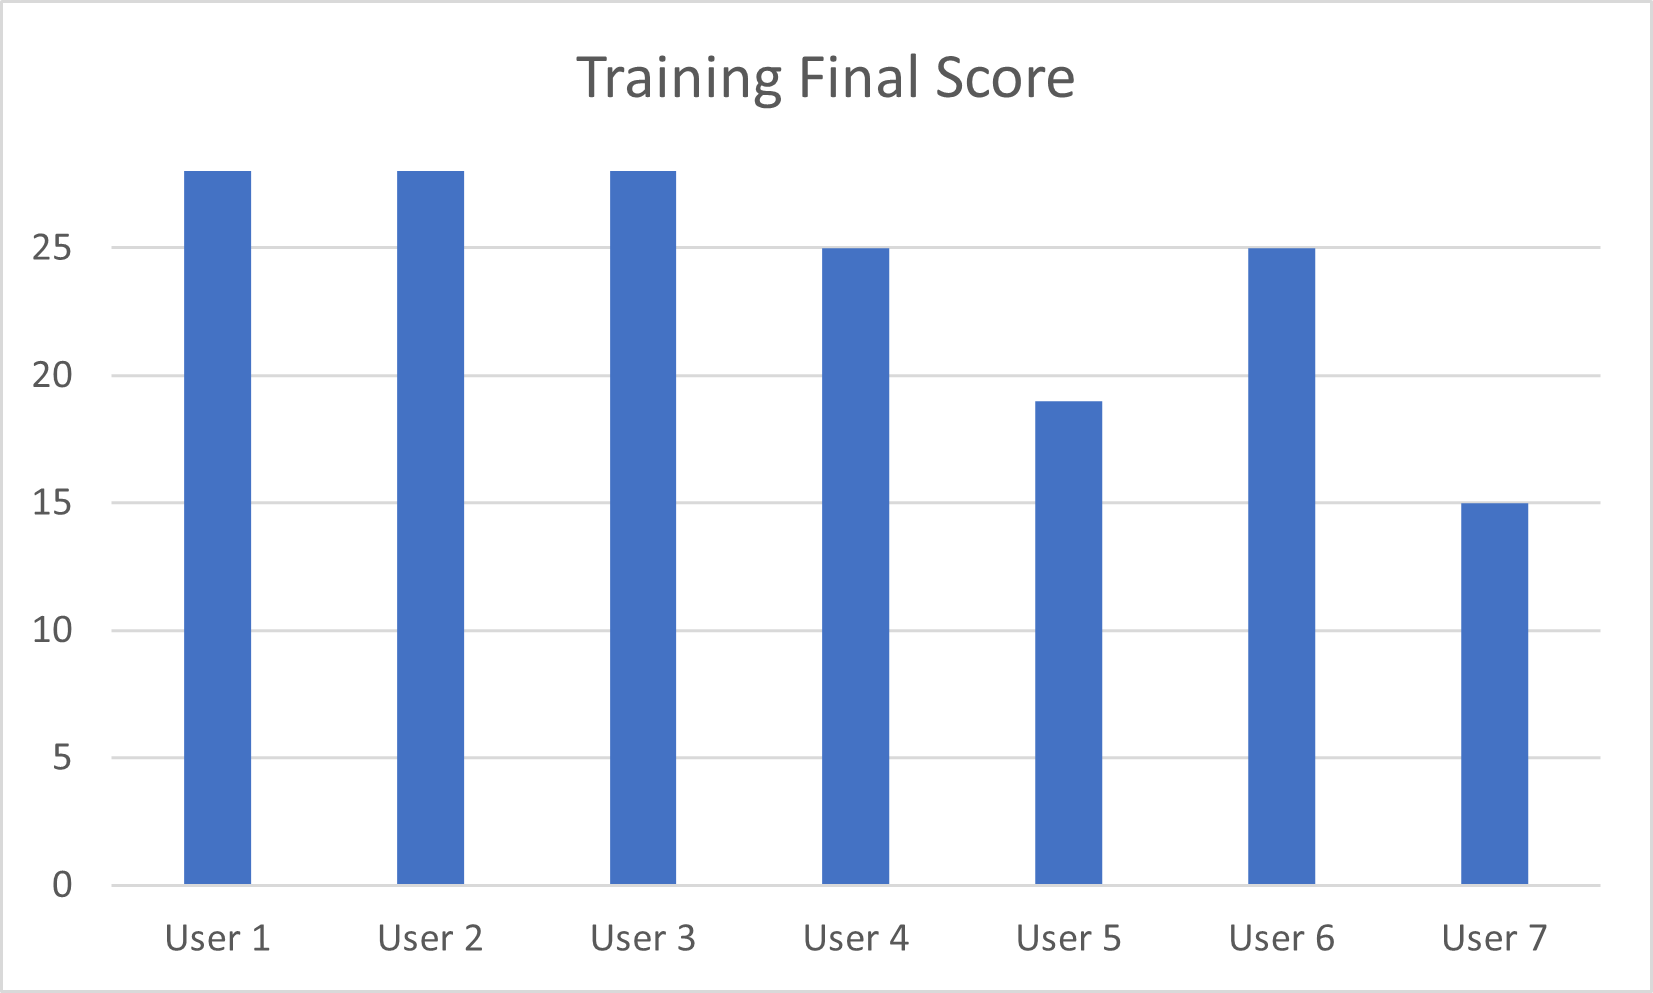
\includegraphics[width=1\linewidth]{images/training_score.png}}
    \caption{Final scores of participants at the end of training}
    \label{fig:training_score}
\end{figure}

\begin{figure}[H]
    \centering
    \frame{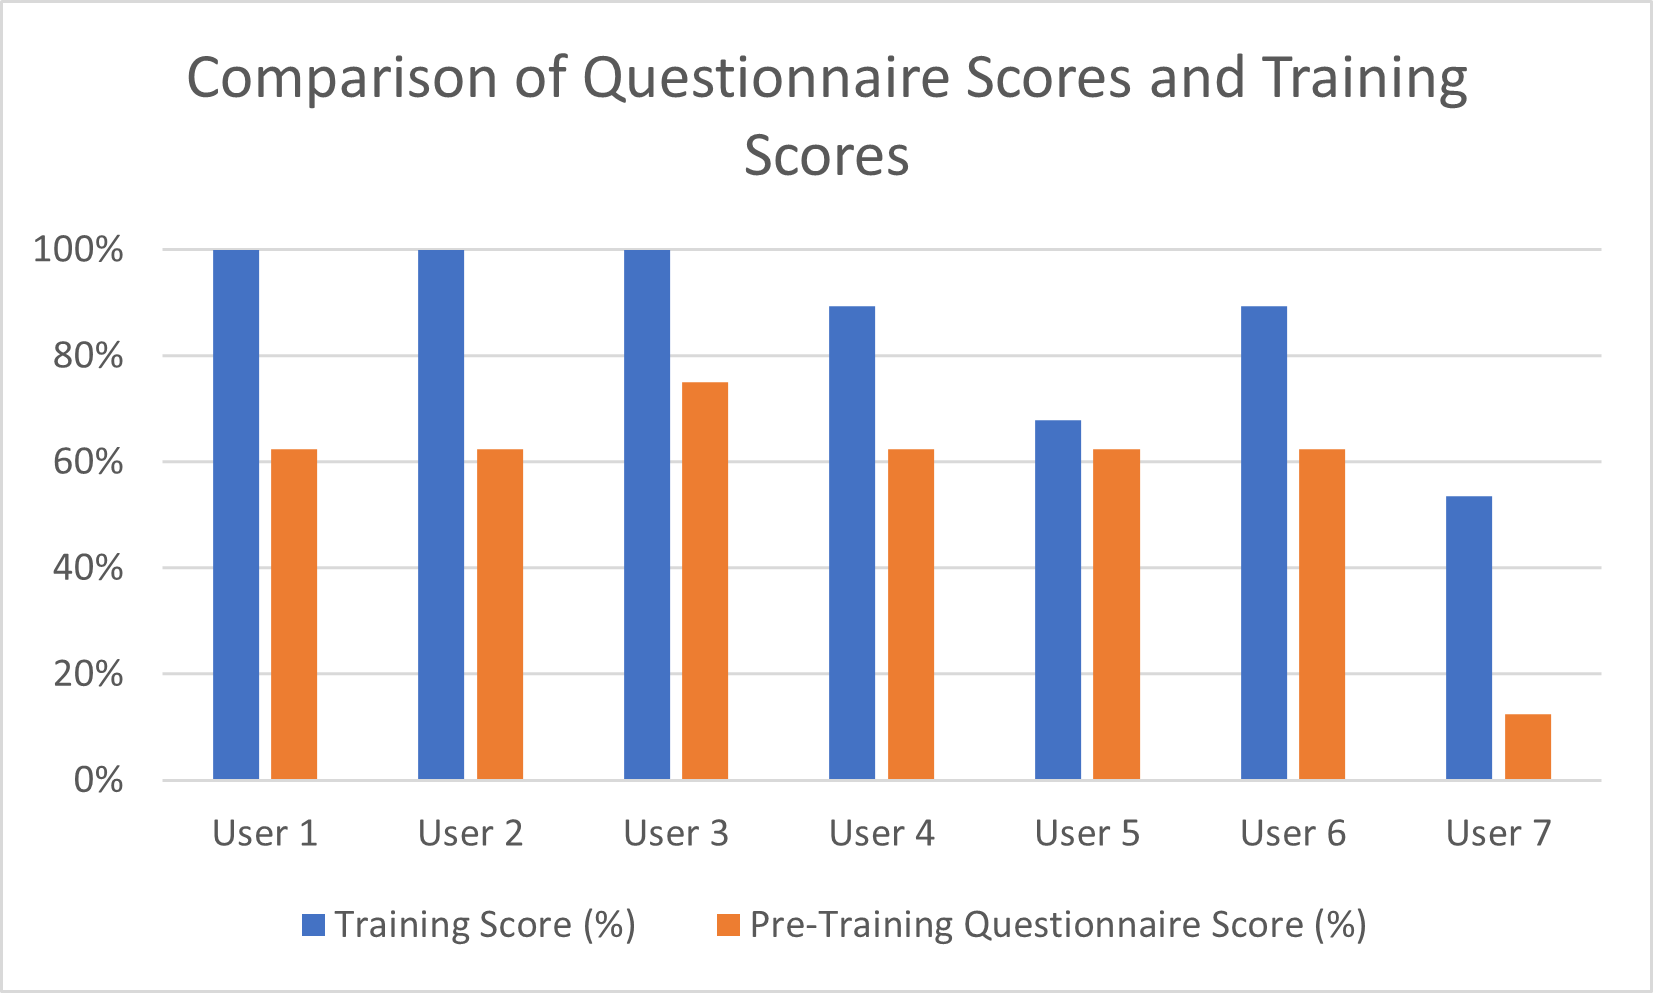
\includegraphics[width=1\linewidth]{images/score_comp.png}}
    \caption{Final training scores of participants compared with their initial questionnaire score}
    \label{fig:score_comp}
\end{figure}

Following the training, the participants were asked to complete the test section of the questionnaire for a second time. It was expected that the training application will have improved their scores in the questionnaire. On average, the second attempt at the questionnaire, the participant score was 5.57 which is a higher average than the previous attempt. Figure~\ref{fig:ques_score_comp} shows the comparison between the two sets of questionnaire results. Despite the rise in average scoring, 4 participants scored exactly the same as their initial questionnaire results. This, once again, shows that the training may not have been difficult enough and may not have taught as many advanced tactics as one would have hoped.

\begin{figure}[H]
    \centering
    \frame{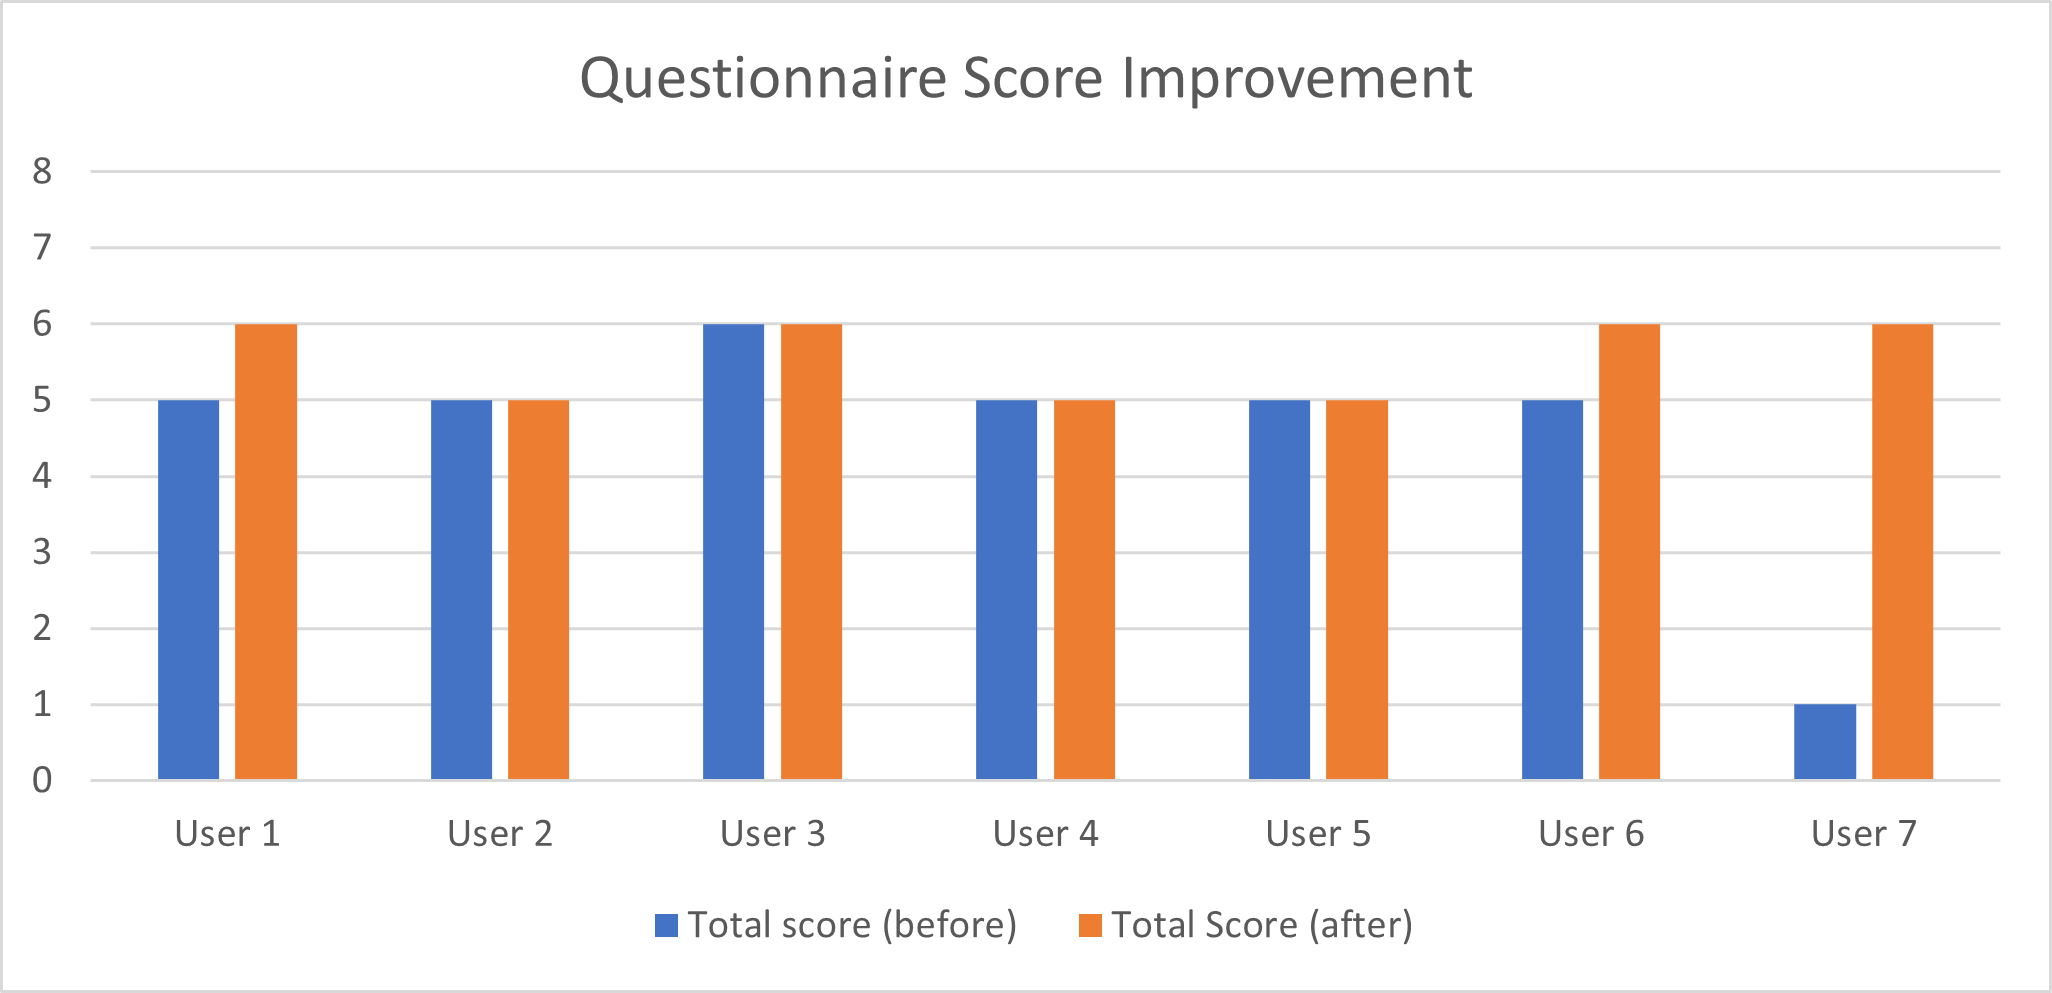
\includegraphics[width=1\linewidth]{images/ques_score_comp.png}}
    \caption{Pre-Training scores of participants compared with their Post-Training Scores}
    \label{fig:ques_score_comp}
\end{figure}


%==================================================================================================================================
\chapter{Conclusion}    

This chapter will summarise the project and achievements made throughout development. It will also reflect on the development process and introduces development concepts that could be use to improve this application in the future.

\section{Summary}
This project attempted to create an effective context-aware training program. As shown by research, the training would focus on employees within a business as the primary target of phishing attacks. This would be applicable to both experienced and inexperienced users. The application is context aware in terms of being applicable to real-world environments and scenarios while also teaching the user about tactics and methods employed by phishers in a safe environment. As shown by the results of the user evaluation, the training material used by the application is also effective and informative. 

\section{Reflection}
Over the course of this project, new experience was gained through the efficient planning, designing, and implementing a large application as an individual developer. The implementation of a full stack web application made use of numerous technologies and extensions, only building on this experience in development and integration.

Despite these benefits, some aspects of the project could have performed better in hindsight. One example of this is the user evaluation, as more time could have been used to run multiple participant experiments while improving the application and training materials based on the feedback received. As a result, the final user evaluation would have most likely shown a greater improvement in the scoring for each of the participants and only improved the training application further. Unfortunately, issues with the COVID-19 pandemic and resulting health concerns hindered the ability to recruit a large enough number of participants to effectively evaluate the project. 

\section{Future Work}
As mentioned previously, some work on the technologies could have been done, such as the use of AngularJS in implementing the single-page application. This would have given the developer a greater level of experience in modern software engineering practices and modern technologies. The replayability of the training game could have also been improved, as the same emails will be shown on the same levels each time it is played. This could be improved in a number of ways:

\begin{itemize}
    \item \verb|Increase number of potential emails|: This would allow a random set of emails to be fetched for each level, decreasing the probability of the same email appearing on multiple playthroughs.
    \item \verb|Auto-generated emails|: This would make use of machine learning to randomly generate phishing emails to be presented to the user on each level. This would require a much greater amount of time to implement but would greatly improve the training effectiveness of the application.
\end{itemize}

%==================================================================================================================================
%
% 
%==================================================================================================================================
%  APPENDICES  

\begin{appendices}

\chapter{Appendices}

\begin{figure}[H]
    \centering
    \frame{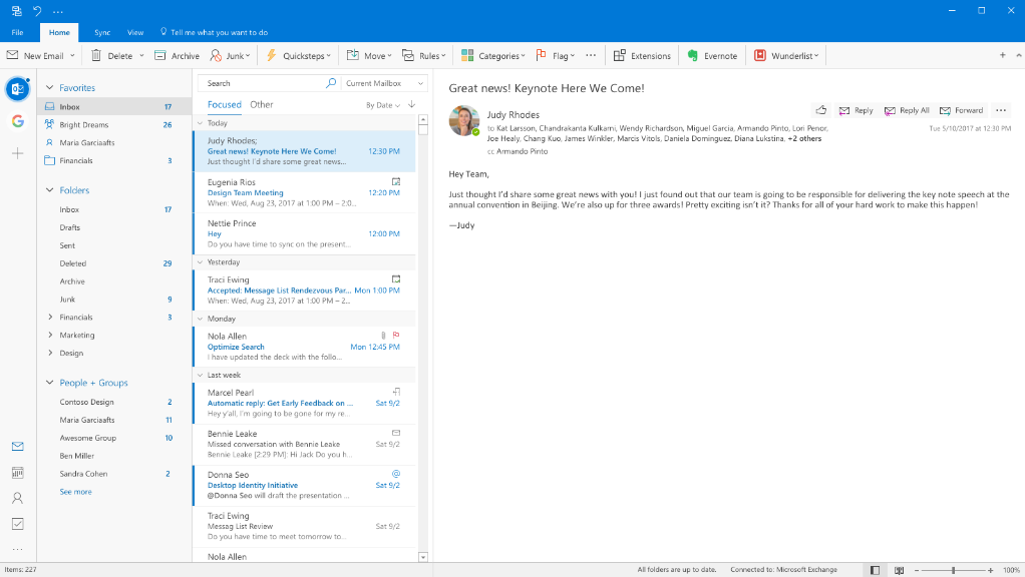
\includegraphics[width=1\linewidth]{images/outlook.png}}
    \caption{Outlook email client}
    \label{fig:outlook}
\end{figure}



\begin{figure}[H]
    \frame{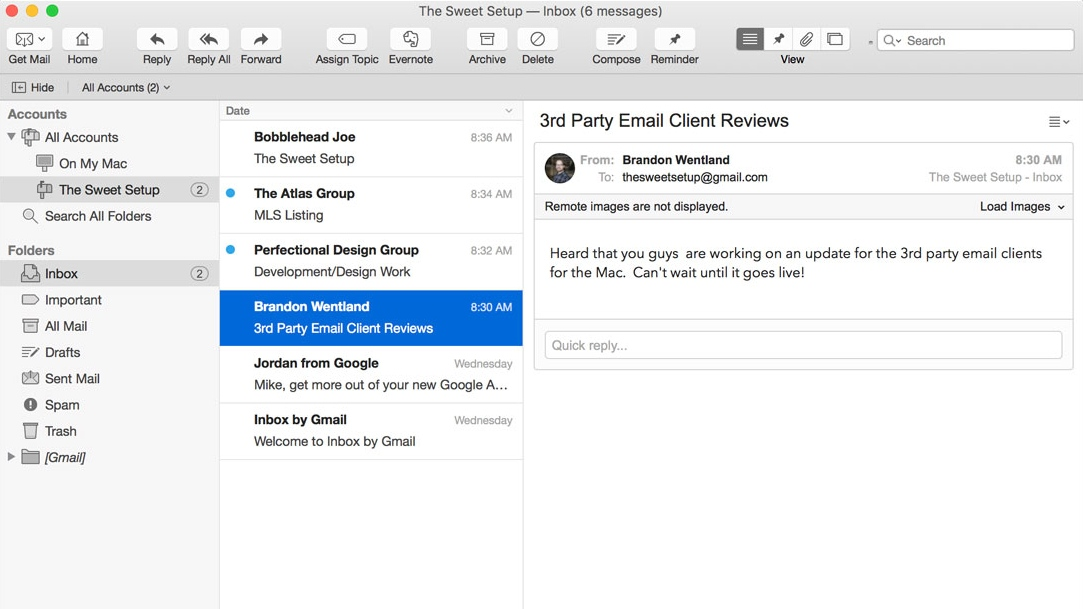
\includegraphics[width=1\linewidth]{images/applemail.png}}
    \caption{Apple Mail desktop email client}
    \label{fig:applemail}
\end{figure}



\begin{figure}[H]
    \frame{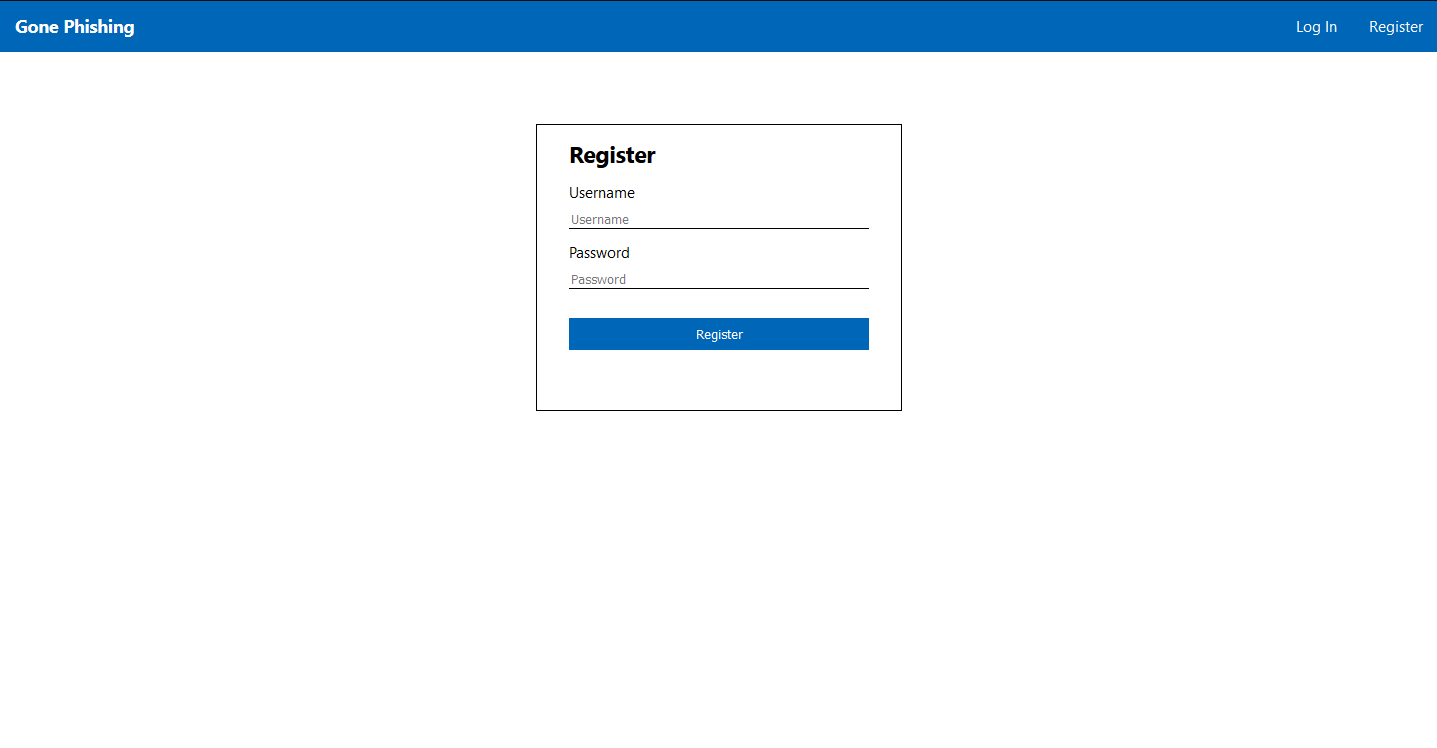
\includegraphics[width=1\linewidth]{images/register_page.png}}
    \caption{Registration Page}
    \label{fig:registration_page}
\end{figure}



\begin{figure}[H]
    \frame{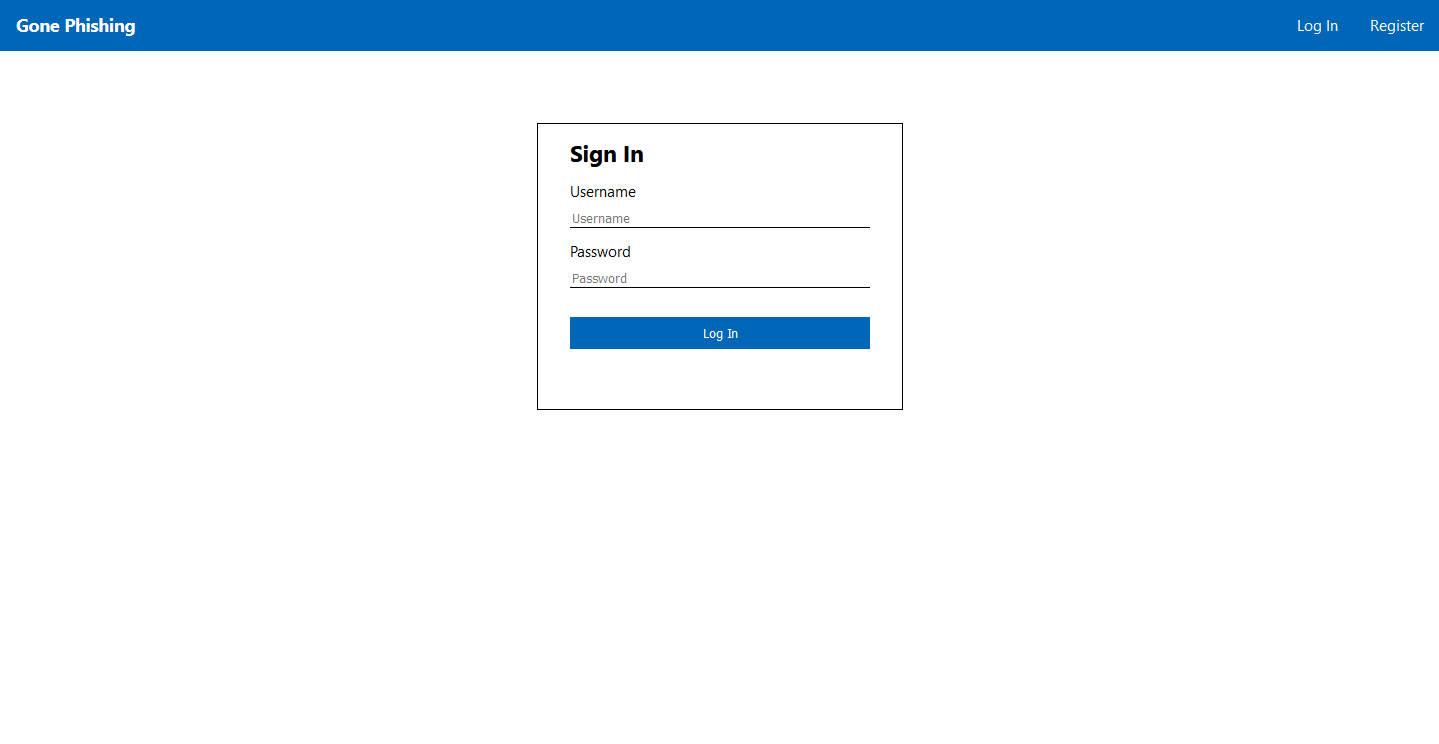
\includegraphics[width=1\linewidth]{images/log_in_page.png}}
    \caption{Log In Page}
    \label{fig:log_in_page}
\end{figure}


\begin{figure}[H]
    \frame{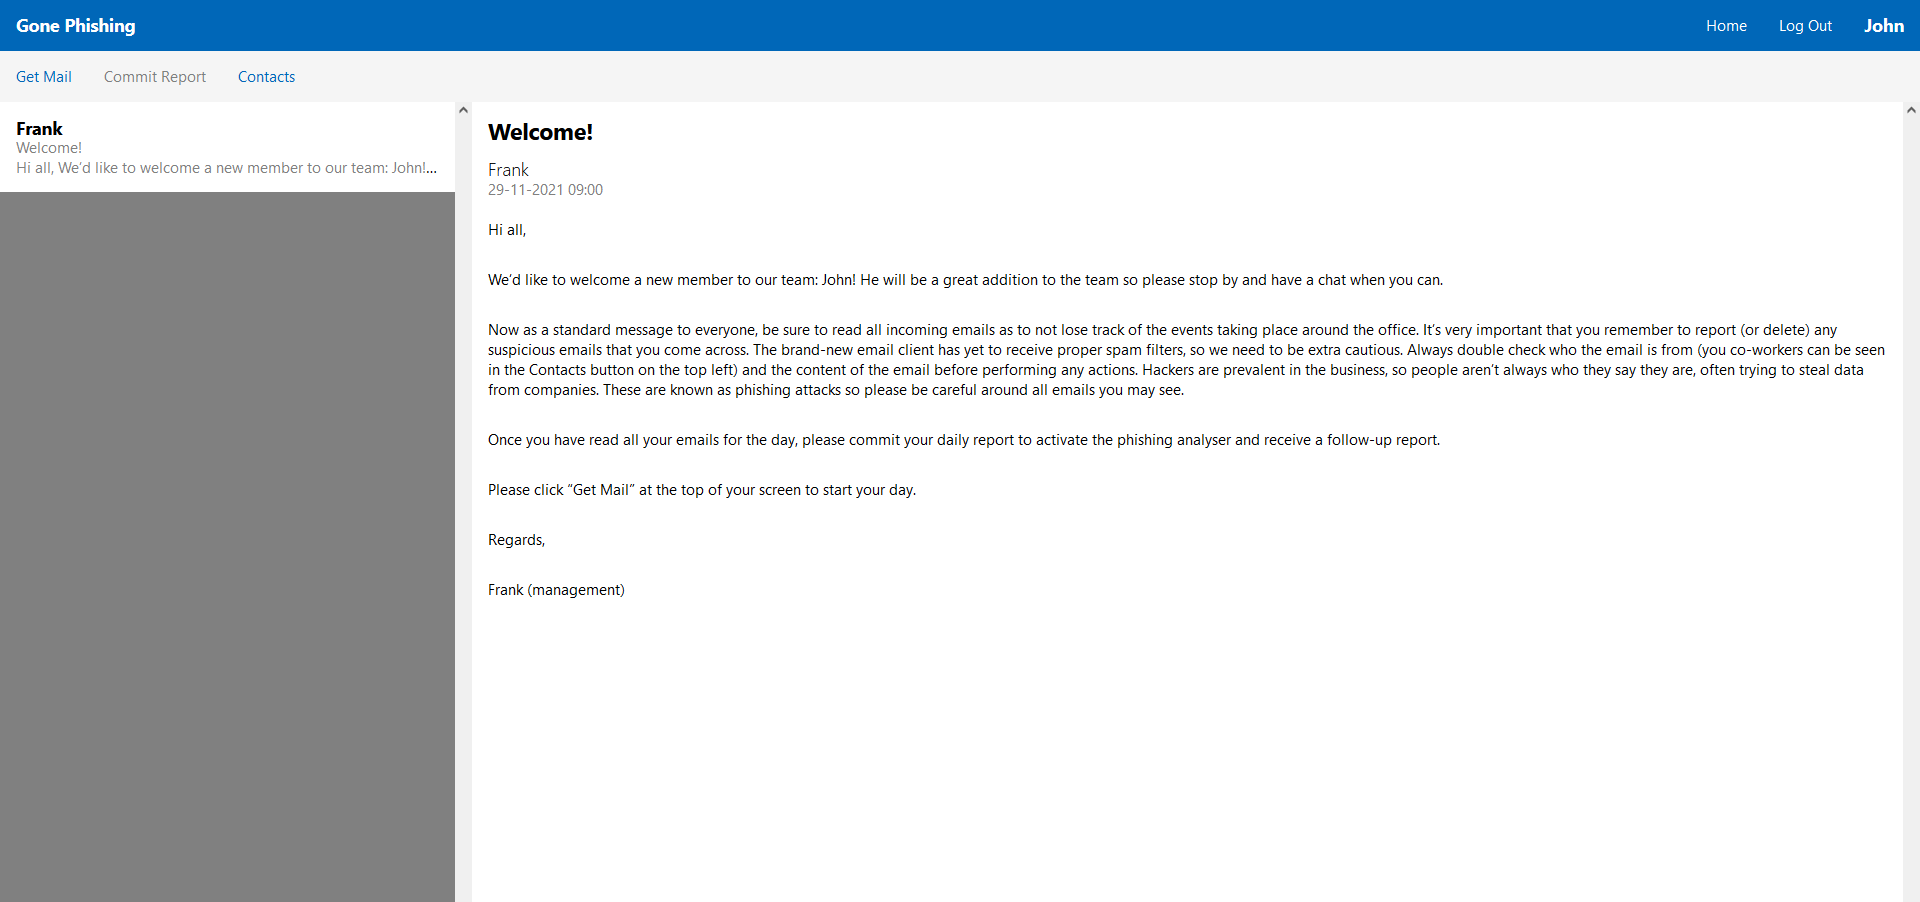
\includegraphics[width=1\linewidth]{images/intro_final.png}}
    \caption{Final implementation of introduction email for level one}
    \label{fig:intro_final}
\end{figure}

\begin{figure}[H]
    \frame{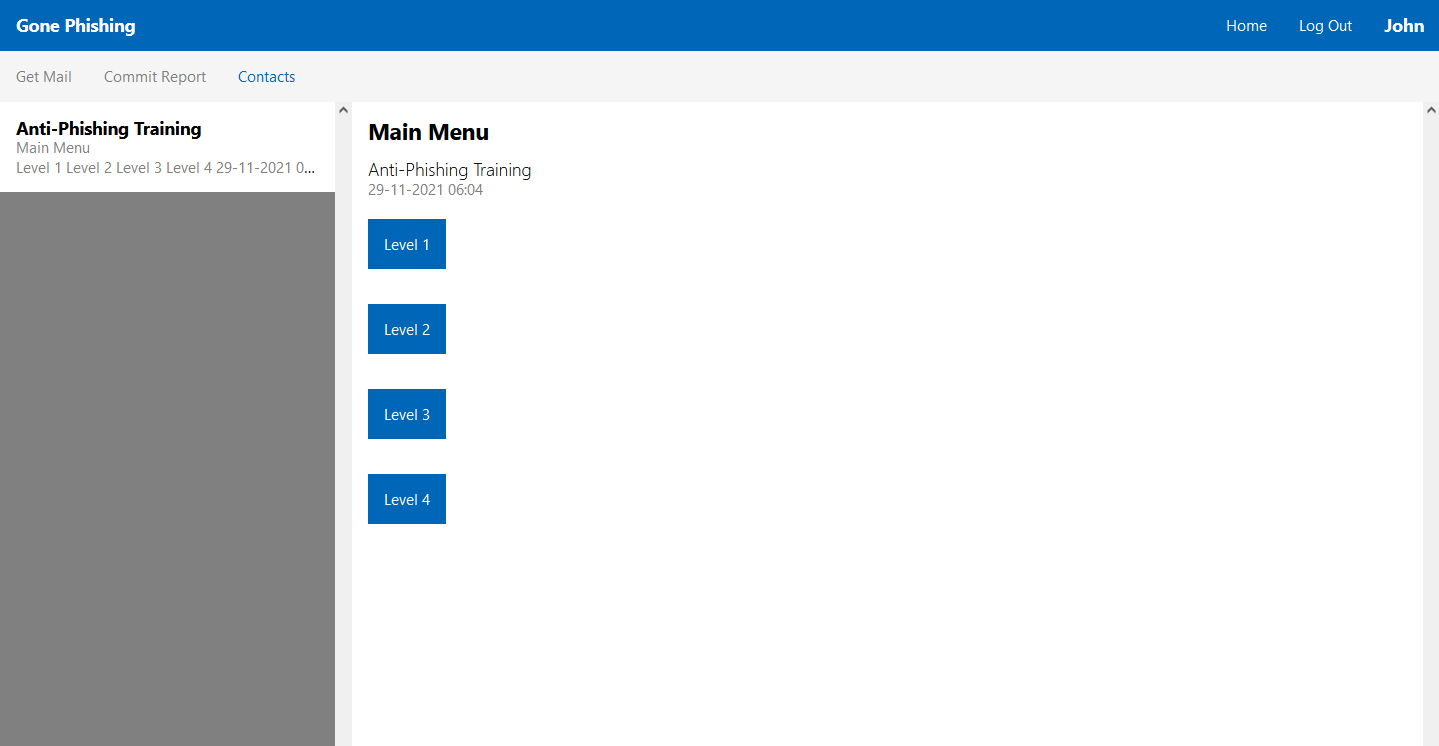
\includegraphics[width=1\linewidth]{images/menu_final.png}}
    \caption{Final implementation of main menu screen}
    \label{fig:menu_final}
\end{figure}

\begin{figure}[H]
    \frame{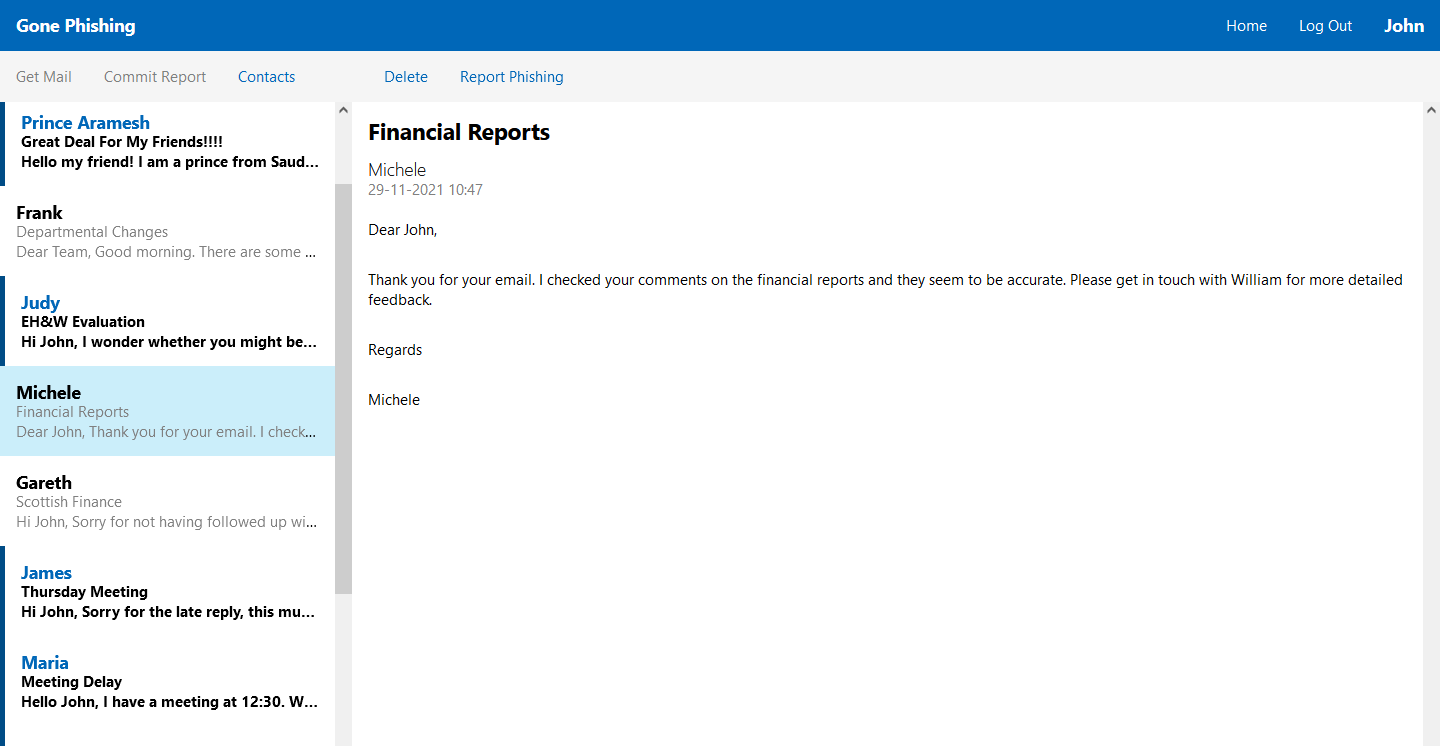
\includegraphics[width=1\linewidth]{images/email_final.png}}
    \caption{Final implementation of main level screen}
    \label{fig:email_final}
\end{figure}

\begin{figure}[H]
    \frame{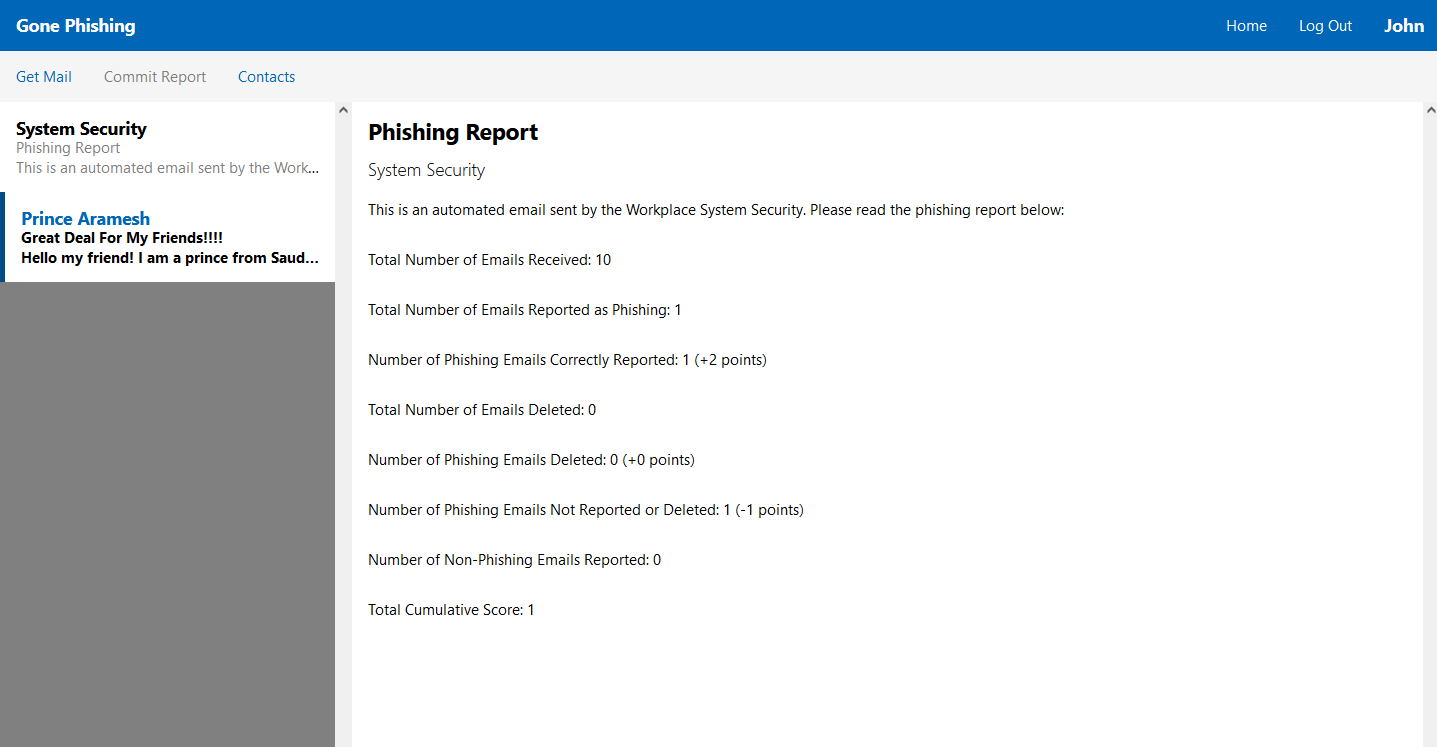
\includegraphics[width=1\linewidth]{images/summary_final.png}}
    \caption{Final implementation of summary screen}
    \label{fig:summary_final}
\end{figure}

\begin{figure}[H]
    \frame{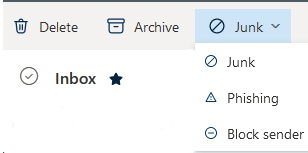
\includegraphics[width=1\linewidth]{images/outlook_report.png}}
    \caption{Report as phishing and delete buttons on the Outlook interface}
    \label{fig:outlook_report}
\end{figure}

\begin{figure}[H]
    \frame{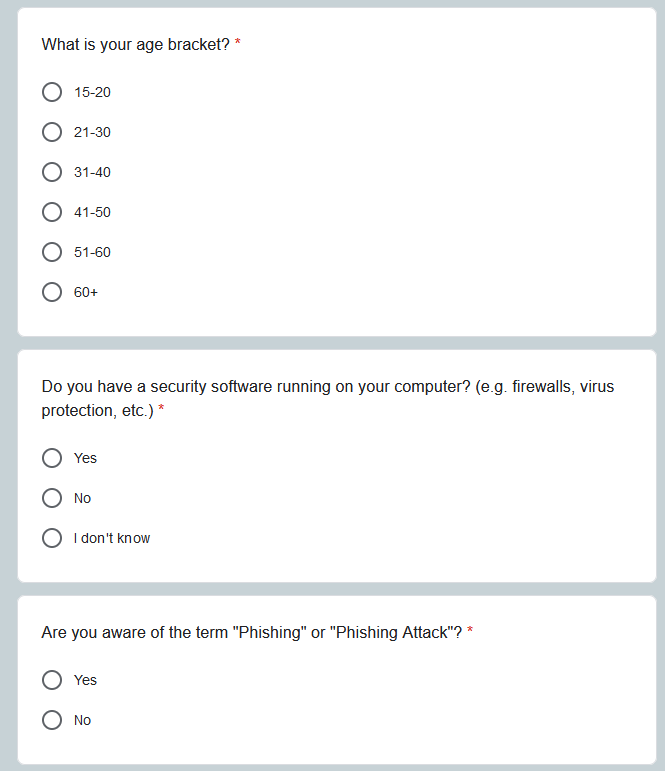
\includegraphics[width=1\linewidth]{images/ques_1.png}}
    \caption{Questionnaire (1)}
    \label{fig:ques_1}
\end{figure}

\begin{figure}[H]
    \frame{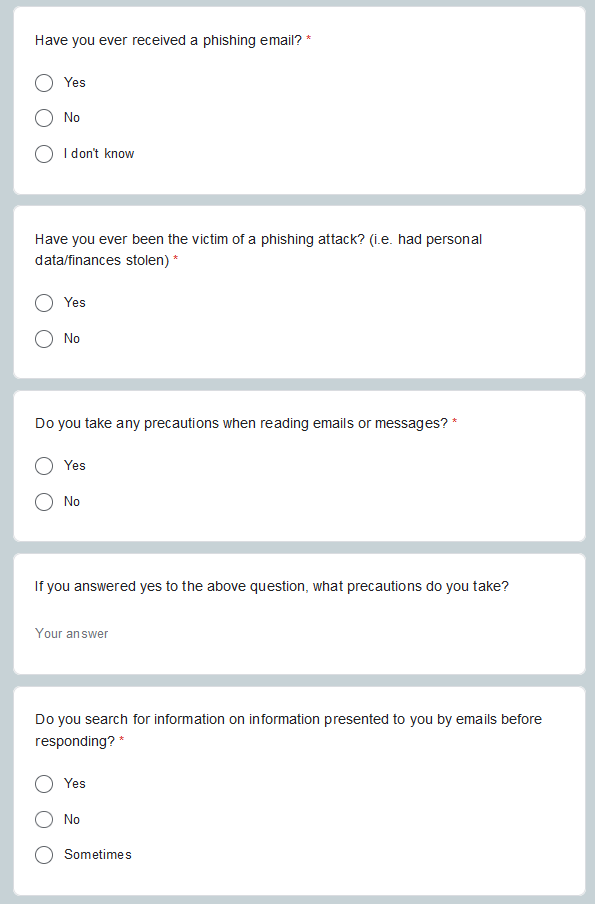
\includegraphics[width=1\linewidth]{images/ques_2.png}}
    \caption{Questionnaire (2)}
    \label{fig:ques_2}
\end{figure}

\begin{figure}[H]
    \frame{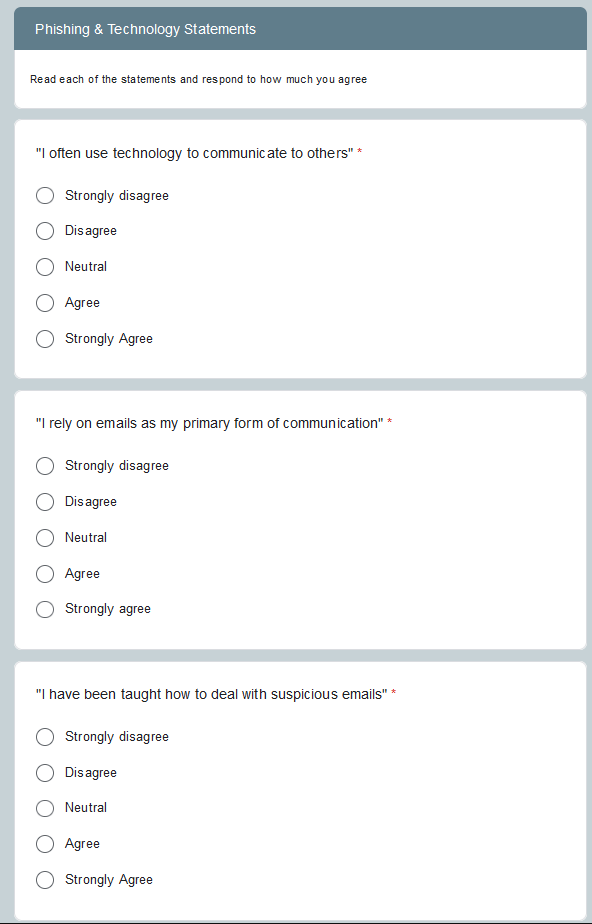
\includegraphics[width=1\linewidth]{images/ques_3.png}}
    \caption{Questionnaire (3)}
    \label{fig:ques_3}
\end{figure}

\begin{figure}[H]
    \frame{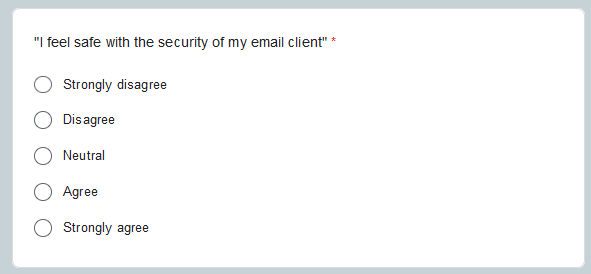
\includegraphics[width=1\linewidth]{images/ques_4.png}}
    \caption{Questionnaire (4)}
    \label{fig:ques_4}
\end{figure}

\begin{figure}[H]
    \frame{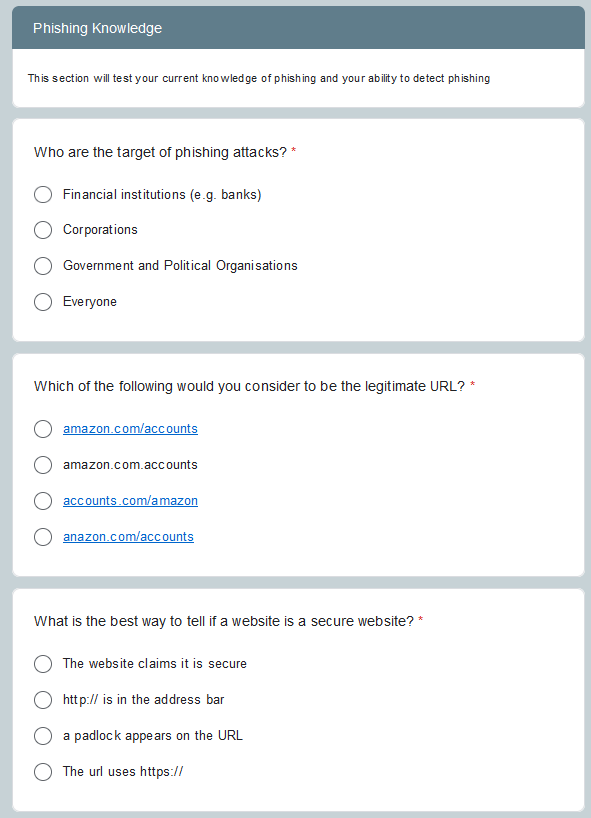
\includegraphics[width=1\linewidth]{images/ques_5.png}}
    \caption{Questionnaire (5)}
    \label{fig:ques_5}
\end{figure}

\begin{figure}[H]
    \frame{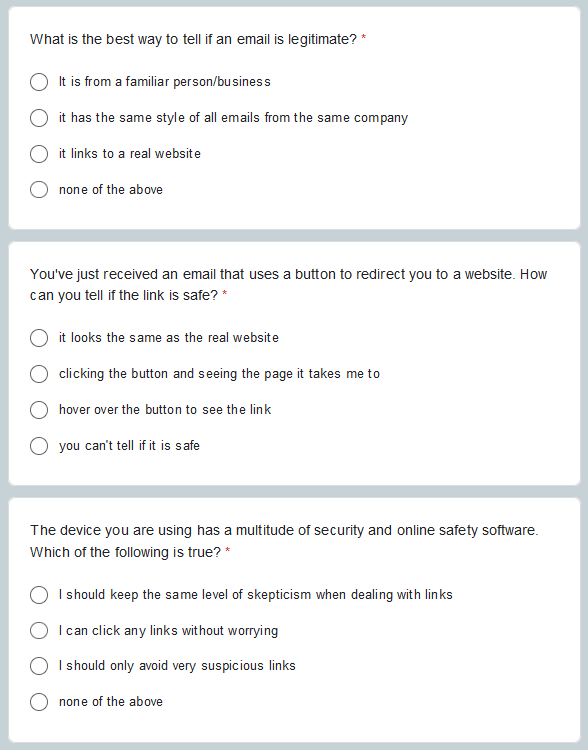
\includegraphics[width=1\linewidth]{images/ques_6.png}}
    \caption{Questionnaire (6)}
    \label{fig:ques_6}
\end{figure}

\begin{figure}[H]
    \frame{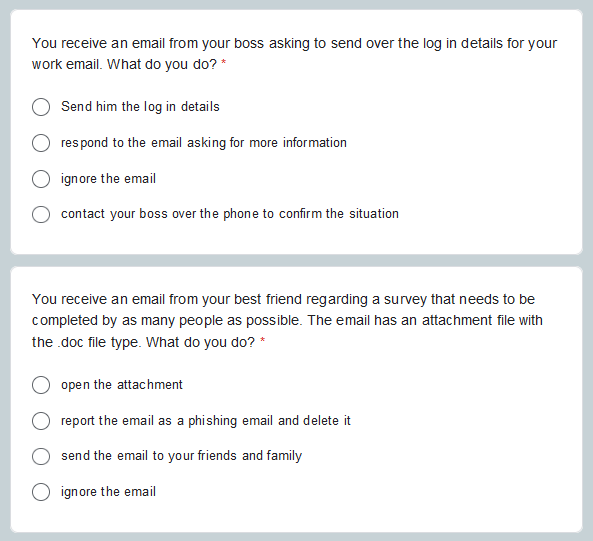
\includegraphics[width=1\linewidth]{images/ques_7.png}}
    \caption{Questionnaire (7)}
    \label{fig:ques_7}
\end{figure}

\begin{figure}[H]
    \frame{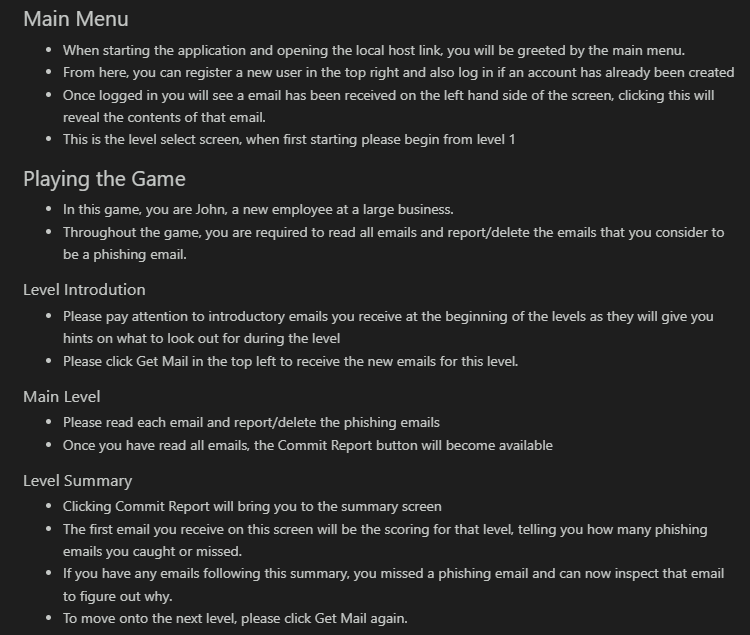
\includegraphics[width=1\linewidth]{images/manual.png}}
    \caption{Manual}
    \label{fig:manual}
\end{figure}

\begin{figure}[H]
    \frame{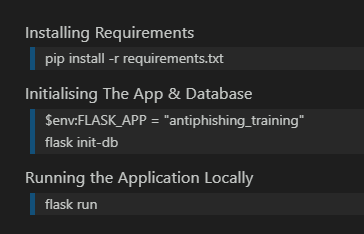
\includegraphics[width=1\linewidth]{images/readme.png}}
    \caption{README.md}
    \label{fig:readme}
\end{figure}
\clearpage

\begin{figure}
    \frame{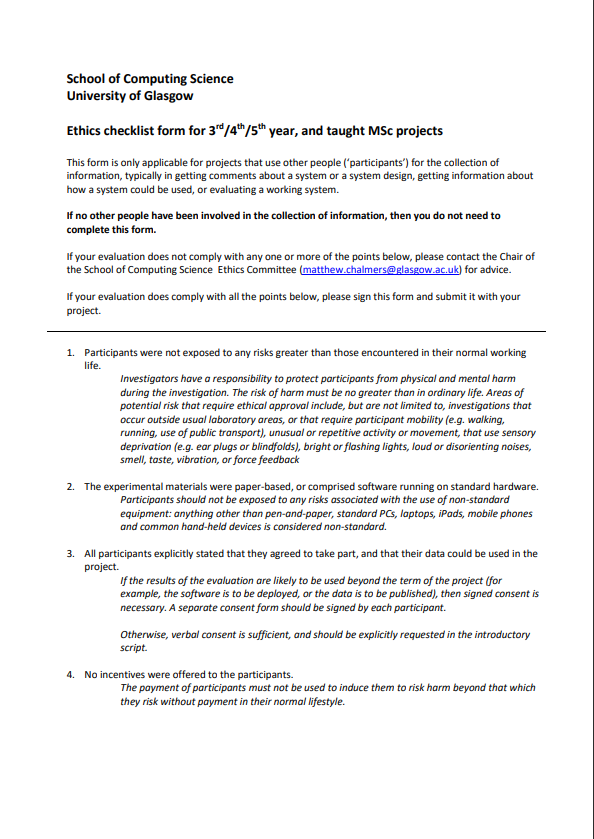
\includegraphics[width=1\linewidth]{images/ethics_1.png}}
    \caption{Ethics Checklist Page 1}
    \label{fig:ethics_1}
\end{figure}

\begin{figure}
    \frame{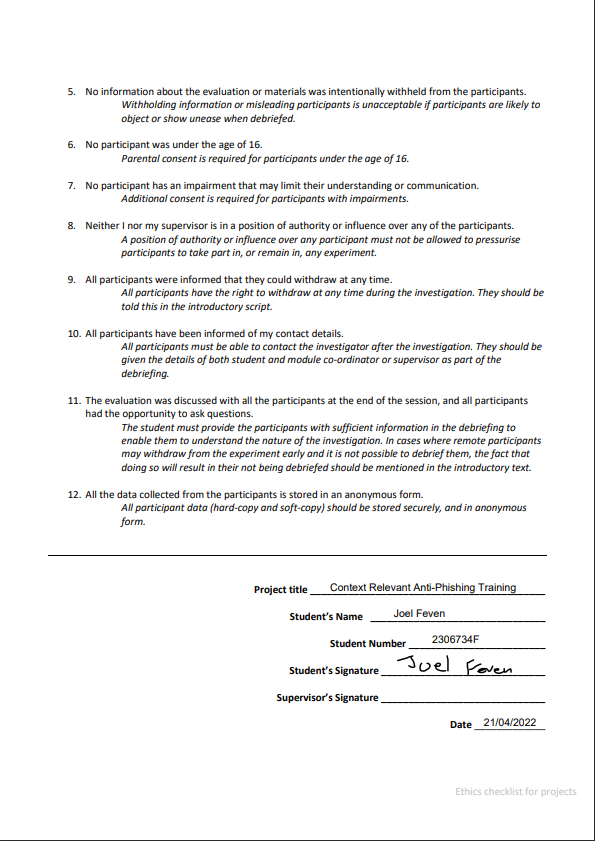
\includegraphics[width=1\linewidth]{images/ethics_2.png}}
    \caption{Ethics Checklist Page 2}
    \label{fig:ethics_2}
\end{figure}

\end{appendices}

%==================================================================================================================================
%   BIBLIOGRAPHY   

% The bibliography style is abbrvnat
% The bibliography always appears last, after the appendices.

\bibliographystyle{abbrvnat}

\bibliography{l4proj}

\end{document}
